\documentclass[11pt, a4paper]{article}

\usepackage[a4paper, margin=2.5cm]{geometry}
\usepackage{fontspec}
\usepackage[english, bidi=basic, provide=*]{babel}
\babelprovide[import, onchar=ids fonts]{english}
\babelfont{rm}{Noto Sans}

\usepackage{amsmath}
\usepackage{booktabs}
\usepackage{array}
\usepackage{tabularx}
\usepackage{longtable}
\usepackage{xcolor}
\usepackage{graphicx}
\usepackage[font=small]{caption}
\usepackage{enumitem}
\usepackage{xurl}
\usepackage{seqsplit}
\urlstyle{tt}
\makeatletter\def\UrlBreaks{\do\/\do\_\do\.\do\-}\def\UrlBigBreaks{}\makeatother\Urlmuskip=0mu\relax
\usepackage[hidelinks]{hyperref}

\definecolor{navy}{HTML}{1B365D}
\definecolor{slate}{HTML}{4A5568}
\definecolor{rulegray}{HTML}{CBD5E0}
\definecolor{panelbg}{HTML}{F7FAFC}

\hypersetup{
    colorlinks=true,
    linkcolor=navy,
    urlcolor=navy,
    citecolor=navy,
    pdftitle={Mitochondrial tRNA-Tyr C33 in four fish lineages occurs without a genome-wide signature of UAA-to-tyrosine reassignment},
    pdfauthor={Thomas Biondi}
}

\linespread{1.08}
\emergencystretch=4em
\setlength{\parskip}{0.45em}
\setlength{\parindent}{0pt}

\begin{document}

% --- TITLE BLOCK ---
{\noindent\small\color{slate}\textbf{PREPRINT} \quad|\quad Evolutionary Biology / Genomics \quad|\quad Pre-registered Study (v4 draft)}
\vspace{0.35em}
{\color{rulegray}\hrule height 0.8pt}
\vspace{1.0em}

{\LARGE\bfseries\color{navy}\raggedright
Mitochondrial tRNA-Tyr C33 in four fish lineages occurs without a genome-wide signature of UAA-to-tyrosine reassignment\par}

\vspace{0.9em}
{\large\textbf{Thomas Biondi}$^{*}$}

\vspace{0.3em}
{\small\color{slate}
Independent Researcher\\
$^{*}$Corresponding author: \href{mailto:tcb.dna@gmail.com}{tcb.dna@gmail.com}
}

\vspace{0.6em}
{\footnotesize\color{slate}
\textbf{Pre-registration:} \texttt{PREREG.md}, SHA-256 \texttt{\seqsplit{e23bc13f37ca48647b86cdc6b3d70abc5f7e0b69c71968de05e7b32285b4fa0c}} (locked 2026-11-23, commit \texttt{5aa5774}).\\
\textbf{Code \& Data:} \url{https://github.com/tcbDNA/tbiondi-genomics/tree/main/metazoan-mito-uaa-tyr} (commit \texttt{35bf5df}).\\
\textbf{Labels used in headings and tables:} \texttt{[C]} pre-registered confirmatory analysis; \texttt{[E]} pre-planned exploratory analysis; \texttt{[S]} the pre-registered weak tier, reported for sensitivity only; \texttt{[P]} post hoc, designed after the screen results were seen.
}

\vspace{0.8em}
{\color{rulegray}\hrule height 0.5pt}
\vspace{0.8em}

% --- ABSTRACT ---
\section*{Abstract}
Lin et al.\ (2026) reported that in bivalves a C at position 33 (C33) of mitochondrial tRNA-Tyr(GUA) occurs only in lineages that read the stop codon UAA as tyrosine, not under the invertebrate code. Satoh et al.\ (2016) had tabulated C33 in 2 of 250 fish mitogenomes without comment. What do the genes and transcripts of fish with C33 show about how they use UAA? A pre-registered screen of 32,982 animal mitogenomes found 17 non-U33 genomes among 28,583 that use UAA as a stop and have a confidently called tRNA-Tyr. In analyses designed after the screen, six fish from four lineages (three sawtooth eels, a bonefish, an eelpout and a danionin minnow) have independent same-species support for C33. None has an in-frame UAA inside its aligned genes, including at 71--72 conserved tyrosine sites; in each, 11 or 12 of 13 genes end in UAA or in a T or TA that polyadenylation would complete. Poly(A) tails show transcripts ending in UAA for seven genes in the bonefish and six in the eelpout, the latter from the sequenced fish. A contig search that finds a hidden second tRNA-Tyr in the nematode \textit{Globodera ellingtonae} found none in the fish above about half the mitochondrial depth. C33 alone therefore does not mark UAA reassignment under the vertebrate code; the bonefish and eelpout keep threonine at position 216 of the release factor mtRF1a. Of the 28,583, the 16,902 using the invertebrate code, including 489 bivalves, have no confirmed C33. The screen confirmed no new reassigned clade, but it recognized only 14 of 20 control genomes known to reassign UAA.

\vspace{0.5em}
\noindent\textbf{Keywords:} mitochondrial genetic code, codon reassignment, tRNA-Tyr, mtRF1a, comparative mitogenomics, pre-registration

% --- INTRODUCTION ---
\section{Introduction}
Animal mitochondria have departed from the standard genetic code many times. One recurring change turns the stop codon UAA into a codon for tyrosine. It has been documented in pterobranch hemichordates (\textit{Cephalodiscus}, NCBI translation table 33; Li et al.\ 2019), plant-parasitic nematodes of the genus \textit{Radopholus} (Jacob et al.\ 2009), tanaidacean crustaceans (\textit{Pseudotanais}; Jakiel et al.\ 2025; Matsushima et al.\ 2026), and several clades of pteriomorphian bivalves in the families Anomiidae, Placunidae and Plicatulidae (Lin et al.\ 2026; Zhao et al.\ 2026). How a stop codon comes to be read as an amino acid without readthrough at every gene that ends in it, and whether the same molecular changes recur in each lineage, are open questions.

Two recent studies pointed to the same tRNA. Lin et al.\ (2026) compared bivalve mitogenomes and found a U-to-C change in the anticodon loop of tRNA-Tyr(GUA). They call it ``U36C'' in their alignment numbering; we infer that it is canonical position 33. In their data, C33 occurs only in lineages that read UAA as tyrosine and is absent from every bivalve that keeps the invertebrate mitochondrial code (NCBI translation table 5, code 5 below), under which UAA is a stop. Zhao et al.\ (2026) reported parallel U33C substitutions in tRNA-Tyr across several reassigned lineages, together with a parallel threonine-to-serine change in the mitochondrial release factor mtRF1a (their T191S, which corresponds to T216S in human \texttt{NP\_061914.3}), and linked reassignment to parallel changes in both. They noted exceptions in \textit{Radopholus similis} and \textit{Pseudotanais}.

Position 33 lies immediately 5$'$ of the anticodon, next to the wobble base G34, which pairs with the third position of the codon. Two effects have been proposed for the substitutions. C33 is predicted to block recognition by tRNA-guanine transglycosylase (TGT), the enzyme that converts G34 to queuosine, so the tRNA would lose the modification of its wobble base. Position 216 lies in the codon-recognition loop of mtRF1a, the release factor that ends translation at UAA, and Zhao et al.\ proposed from structural modeling that T191S in mtRF1a (T216S here) could weaken recognition of UAA. If the two changes must occur together, a genome could carry C33 beside an unchanged release factor and still use UAA as a stop.

C33 had already been recorded in fish. Satoh et al.\ (2016) tabulated the base at every tRNA position in 250 fish mitogenomes. Their Table S7 gives C at position 33 of tRNA-Tyr (position 39 in their numbering) in 2 of the 250 and T in 248, without naming the two species or discussing them. Two records in their species list carry C33 in our calls, both from bonefishes: \texttt{AP002973}, filed as \textit{Albula glossodonta}, and \textit{Pterothrissus gissu} (\texttt{AB051197}, the source of \texttt{NC\_005796}). We infer that these are the two. Li et al.\ (2019) also stated that starfish, which keep UAA as a stop under the echinoderm code (code 9), carry C at position 33 of tRNA-Tyr, whereas Zhao et al.\ depict U33 in \textit{Asterias rubens}.

These observations raise a straightforward question: when a fish carries C33, what do its mitochondrial coding sequences and transcript ends show about how it uses UAA? If UAA were read as tyrosine throughout a genome, it would appear inside genes, some of it where related species have a conserved tyrosine, and genes would not end in it, because a ribosome reading UAA as tyrosine would continue past it. We put this question to six fish from four lineages, found in a pre-registered screen of 32,982 public animal mitogenomes. The screen was designed to find new UAA-to-tyrosine reassignments and to test whether a base other than U33 in tRNA-Tyr accompanies them. Its rules were fixed before any genome outside the control panel (360 genomes of known code, used for calibration) was screened; the analyses of the fish were designed afterwards. For each fish we ask where UAA occurs in its genes and mature transcripts, whether other records or individuals of the same species carry C33, whether a second mitochondrial tRNA-Tyr could be hidden, and whether its mtRF1a keeps the canonical residue at position 216. We also report what the screen shows for invertebrates using code 5, the setting of Lin et al.'s observation, and for two other genera it flagged: \textit{Craniella} sponges, which carry G33, and the nematode \textit{Rotylenchulus reniformis}, a candidate reassignment.

% --- RESULTS ---
\section{Results}

\subsection{A pre-registered screen finds non-U33 tRNA-Tyr in 17 genomes that use UAA as a stop \texttt{[C]}}\label{sec:screen}
We screened 32,982 animal mitogenomes from NCBI RefSeq release 238, NCBI organelle assemblies and eligible records of the International Nucleotide Sequence Database Collaboration (INSDC). Of these, 32,623 are confirmatory genomes, used for the pre-registered counts and rates; the rest are records of control-panel species and one bonefish record kept for a targeted test (Methods). Each genome was examined in two ways, by rules fixed in the pre-registration. A classifier decided whether UAA behaves as a stop or as a tyrosine codon, from in-frame UAA codons inside aligned protein-coding genes, particularly at columns where tyrosine is conserved, and from Codetta, a program that predicts the genetic code from nucleotide sequence (Shulgina \& Eddy 2021, 2023). Separately, we called the base at position 33 of tRNA-Tyr(GUA) with a covariance model. A call of a base other than U33, or a weaker U33 hit, also needed a second tRNA finder at the same place, and every call had to pass structural checks of the anticodon stem and of overlaps with other genes (Methods). We call a tRNA-Tyr that passed these checks resolved.

The classifier placed 32,510 confirmatory genomes in the stop class and 1 in the tyrosine class; the others fell into the ambiguous (48), too-little-sequence (61) and weak (3, all rejected on audit) classes. Of the stop-class genomes, 28,583 had a resolved tRNA-Tyr. Codetta made no confident call for 28,580 of these 28,583, so their stop class rests on the count of in-frame UAA. Of the 28,583, 28,566 carried U33 and 17 carried another base, C33 in 14 and G33 in 3 (Table~\ref{tab:hits}, Figure~\ref{fig:tree}): 0.059\% of records. This rate does not estimate how common non-U33 tRNA-Tyr is, because the screen never measured how often it misses a non-U33 base. Thirteen of the 17 are vertebrates using the vertebrate mitochondrial code (code 2; 12 C33 and 1 G33, among 10,717 genomes), two are G33 sponges using the sponge code (code 4; of 150), and two are C33 nematodes using code 5 (of 16,902). None occurred among the 814 genomes using codes 9, 13, 14 or 21 or without an assigned code.

The screen found no new reassigned clade. Its one confirmatory genome in the tyrosine class, the nematode \textit{R.\ reniformis}, failed the anticodon-stem check and therefore could not count as a new clade under the pre-registered rules (Section~\ref{sec:roty}). The screen may also have missed reassigned lineages: with the tRNA checks included, it recognized only 14 of 20 control genomes from known reassigned lineages (Figure~\ref{fig:calib}; Section~\ref{sec:checks}).

\subsection{Gene interiors, gene ends and transcript ends in six C33 fish \texttt{[P]}}\label{sec:fish}
Twelve of the 14 C33 genomes are vertebrates. Six of them, from four lineages of fish, have C33 confirmed in another record or individual of the same species (Section~\ref{sec:support}), and they are the subject of this section: three sawtooth eels (Serrivomeridae: \textit{Serrivomer beanii}, \textit{S.\ sector} and \textit{Stemonidium hypomelas}), an eelpout (Zoarcidae: \textit{Lycenchelys verrillii}), a bonefish (Albulidae: \textit{Albula glossodonta}) and a danionin minnow (Danionidae: \textit{Microdevario kubotai}). All six use the vertebrate mitochondrial code, under which UAA is a stop. The bonefish lineage is the one in which Satoh et al.\ (2016) had tabulated C33. The \textit{A.\ glossodonta} record counted here (\texttt{CM165726.1}) is not their record \texttt{AP002973}, which is filed under the same name but is only 87\% identical to it. The sawtooth eels, the eelpout and the minnow extend C33 to three further lineages.

If UAA were read as tyrosine across these genomes, it would appear inside genes, and genes would not end in it. We examined both in the 13 protein-coding genes of each fish (Table~\ref{tab:sixfish}; Supplementary Table S1). None of the six has an in-frame UAA in the aligned interiors of its genes (3,352--3,398 codons per genome, excluding the first and last 10 codons of each gene). Each has 71 or 72 alignment columns where tyrosine is conserved; 53--58 of these are encoded by UAU or UAC and the rest by other codons, never by UAA.

We used three kinds of evidence about gene ends. In some genes the genome encodes a complete UAA. In others it encodes only T or TA, an incomplete stop that polyadenylation of the transcript completes to UAA (Ojala et al.\ 1981). Where RNA is available, poly(A) tails show where the mature transcript ends and which codon it ends with. Each fish encodes a complete UAA at the end of four to six of its 13 genes and T or TA at the end of six or seven more. UAG ends at most two genes in a fish, and AGA or AGG at most one. The gene ends come from GenBank annotations; for the two unannotated assemblies (\textit{A.\ glossodonta} and \textit{L.\ verrillii}) we transferred them from other records of the same species. Of the 78 ends, 76 agree with the reading frame of the protein alignment and lie within five residues of the median C-terminus of 14 reference fish that carry U33 and use UAA as a stop. The two exceptions are in \textit{S.\ beanii}: \textit{COX1} ends six residues beyond that median, and \textit{ND2} ends in frame but has no tRNA or gene start called at its end to confirm the boundary.

RNA-seq exists for two of the six fish. The \textit{A.\ glossodonta} RNA comes from the liver of another fish of the species (\texttt{SRR13036352}; its identity is checked in Section~\ref{sec:support}). Poly(A) tails, 17--200 reads per gene, place the 3$'$ end of seven transcripts where the mRNA reads UAA in frame. One gene, \textit{COX1}, encodes the complete triplet, and polyadenylation supplies the missing bases in the other six (\textit{ND2}, \textit{ATP6}, \textit{COX3}, \textit{ND3}, \textit{ND4} and \textit{CYTB}). One transcript ends differently: \textit{COX2} ends at the AGG annotated as its stop (132 of 134 tail reads).

The \textit{L.\ verrillii} RNA comes from muscle of the same fish whose mitogenome was screened (\texttt{SRR36303867}), so here the genome and its transcripts describe one animal. Six of its transcripts end in UAA, with 17--110 tail reads each: \textit{ND1} encodes the complete triplet, and polyadenylation completes it in \textit{ND2}, \textit{COX2}, \textit{ATP6}, \textit{COX3} and \textit{CYTB}.

In both fish, the encoded UAA of \textit{ATP8} and \textit{ND4L} lies inside a longer transcript shared with \textit{ATP6} or \textit{ND4}, and the remaining genes had fewer than five tail reads. We found no RNA-seq or transcriptome assemblies for the other four fish; in them, completion of the T and TA ends to UAA is predicted from the genome, not observed.

A ribosome that read UAA as tyrosine would run past the end of 11 or 12 of the 13 genes in each fish. With no UAA inside the genes, this makes a genome-wide reassignment of UAA unlikely in these fish. The RNA establishes the sequence and position of the mature transcript ends, not what a ribosome does there, so rare or context-dependent reading of UAA as tyrosine is not excluded, and termination itself was not measured.

\subsection{Other records and individuals of the same species carry C33 \texttt{[P]}}\label{sec:support}
Some of the 17 hits rest on a single record with no independent support, so after the screen we graded each by the evidence that its base at position 33 is real (Table~\ref{tab:hits}). The grades follow one rule, written after the evidence for all 17 had been seen (Methods). A hit reaches Tier 1 when the record's base appears in a distinct record of the same species, or in at least 10 reads from another individual with at most 1\% U33 observed. Tier 2 requires such reads from the sequenced specimen itself. Tier 3 has no evidence from the same species, but related species agree: in the smallest NCBI taxon that holds another species with a confident call, every such species carries the same base, and at least one of them is Tier 1 or 2. A hit is dropped when the same genome holds a second tRNA-Tyr with a different base that Infernal and ARAGORN place identically, and a hit that meets none of these rules is unconfirmed. Thirteen of the 17 reached Tiers 1--3, three were unconfirmed and one was dropped. The six fish of Section~\ref{sec:fish} are the Tier 1 C33 genomes.

Each of the six fish has C33 in at least one other record or individual of its species, although two rest on weaker records. For five, the support is another GenBank mitogenome, so we checked that these records come from different animals and that the species names are right. Two \textit{Albula} records in GenBank are probably mislabelled, among them \texttt{OZ556087}, filed as \textit{A.\ vulpes} but 99.8--100\% identical in \textit{CYTB} to \textit{A.\ glossodonta}. We compared voucher, BioSample, submitter and collection data and the \textit{COX1} and mitogenome divergence of every comparison record (Supplementary Table S2). No pair was a duplicate or a resubmission, every comparison record carried C33, and each of the five species has at least one comparison record from a distinct specimen (Table~\ref{tab:hits}). The two weaker cases are \textit{S.\ sector} and \textit{M.\ kubotai}. The counted \textit{S.\ sector} record lacks a voucher, its \textit{COX1} group includes one record filed as \textit{S.\ jesperseni}, and one comparison record filed as \textit{Stemonidium} is \textit{S.\ sector} by sequence. For \textit{M.\ kubotai}, Tier 1 rests on \texttt{PV357791}, an independent record of the same species that carries C33 and is 99.9\% identical to the screened record in \textit{COX1}. It lacks a BioSample, so its specimen metadata are incomplete, and four other records filed under the name differ by 2.2--4.6\% in \textit{COX1} and remain unconfirmed as conspecific. The sequencing run used for \textit{M.\ kubotai} in the read and contig searches (\texttt{SRR39401262}) comes from yet another fish. Its assembled mitochondrial contig (16,852 bp) is 97.6\% identical to the screened record (2.4\% divergent) and 99.8\% identical to \texttt{PV357792}, one of the four unconfirmed records, so its species identity is uncertain, and the read counts and second-copy searches for \textit{M.\ kubotai} describe that fish rather than the screened specimen. For \textit{A.\ glossodonta}, the support comes from the RNA-seq run of another fish (\texttt{SRR13036352}), whose \textit{CYTB} is 100\% identical to \texttt{CM165726.1} over 1,110 bp and 82.7\% identical to the Hawaiian endemic \textit{A.\ virgata} (\texttt{KJ910045}).

Reads also limit how much U33 tRNA-Tyr a fish could carry beside C33. The argument needs C33 to be the dominant tRNA-Tyr allele, with no second working copy; it does not need an absence of U33 reads. The tier rule used the observed U33 share. A stricter rule, which requires the exact one-sided 95\% upper bound on that share to be at most 1\% wherever reads carry a tier, leaves all six fish in Tier 1: five through the other GenBank records, and \textit{A.\ glossodonta} through its RNA reads (bound 0.26\%; Table~\ref{tab:summary}; Methods). Under the stricter rule, one of the three Tier 2 eels, \textit{Serrivomer lanceolatoides}, keeps its tier, and \textit{Coloconger meadi}, \textit{Ophichthus asakusae} and both \textit{Craniella} sponges become unconfirmed.

\subsection{A hidden tRNA-Tyr copy in \textit{Globodera}, and the search for one in the fish \texttt{[P]}}\label{sec:glob}
The nematode \textit{Globodera ellingtonae} shows how C33 can mislead. Its mitochondrial genome is split across chromosomes, and the screened record (\texttt{KU726971.1}, chromosome I) carries C33. At that locus, 447 reads from two populations (176 and 271 reads) support C33 and none support U33. Chromosome II (\texttt{KU726972}) nevertheless encodes a second tRNA-Tyr with the canonical U33 (positions 6699--6752), placed identically by Infernal and ARAGORN, and we dropped the genome from the evidence tiers. Reads could not reveal this copy because the two genes share only 19 of 26 aligned bases, so neither exact matching of 31-base words (31-mers) nor a similarity search that starts from the C33 gene reaches it. However many reads support C33 at one locus, they cannot exclude a second copy elsewhere.

Within the six fish records, every second hit with a GUA anticodon was either a tRNA-Thr(UGU) gene on the opposite strand, which the covariance model reads with a one-nucleotide slip, or an antisense call made only by ARAGORN inside \textit{ND4} or \textit{ND5}. In \textit{L.\ verrillii}, a 90,807-bp contig of tandem mitogenome copies (\path{JBQQXK010000041.1}) carries C33 in all five of its \texttt{trnY} copies.

To look beyond the records without relying on similarity to the C33 gene, we searched assembled contigs. Each sequencing library was subsampled to 22--68$\times$ mitochondrial depth and assembled, and every contig of at least 500 bp present at half the mitochondrial coverage or more was searched for tRNA-Tyr with the screen's tRNA caller and with ARAGORN. In \textit{Globodera}, this search recovers chromosome II (68$\times$) as the only contig with a tRNA-Tyr that passes.

In the six fish, the search found no second mitochondrial tRNA-Tyr. \textit{S.\ sector}, \textit{L.\ verrillii}, \textit{M.\ kubotai} and \textit{A.\ glossodonta} returned no passing contig (Table~\ref{tab:hits}). In \textit{S.\ beanii}, the one passing contig is a dispersed nuclear repeat, with 2.9\% median read divergence, 17\% \textit{k}-mer coverage of mitochondrial DNA and no mitochondrial genes. In \textit{St.\ hypomelas}, the three passing contigs are bacterial and phage DNA, identified with Pfam and bacterial-mode tRNAscan-SE (Supplementary Table S3). The search sees only molecules that assemble and are present at about half the mitochondrial depth or more; a copy at lower abundance, or one that does not assemble, would be missed. None of the libraries came from the screened specimens. For \textit{S.\ beanii}, \textit{S.\ sector}, \textit{St.\ hypomelas} and \textit{L.\ verrillii} they are the runs from other individuals listed in Table~\ref{tab:hits}. For \textit{A.\ glossodonta} the library is whole-genome-amplified DNA of a different fish (mitogenome 99.7\% identical to the record), and for \textit{M.\ kubotai} it is \texttt{SRR39401262}, from the fish of uncertain species described in Section~\ref{sec:support} (its 16,852-bp mitochondrial contig is 2.4\% divergent from the screened record), so the search applies to that fish. For these two fish the search used contigs from an intermediate assembly stage, before repeats were resolved.

A read search, which does depend on similarity, complements the contig search. We aligned all reads that match the tRNA-Tyr gene body at 70\% identity or more competitively to tRNA-Tyr, to every other mitochondrial tRNA on both strands and to cytosolic tRNA-Tyr. Across the runs of the seven Tier 1 genomes (the six fish and the sponge \textit{Craniella infrequens}), only five reads carried U33, four of them in the fish, each a singleton with canonical mitochondrial flanks. In each fish's best run, this bounds a minor U33 allele at 0.25--2.81\% (Table~\ref{tab:hits}); for \textit{M.\ kubotai} the bound applies to the \texttt{SRR39401262} fish. In simulations, the search recovers at least 99\% of copies that differ from the C33 gene by 10\%, 91--94\% at 15\%, 65--70\% at 20\% and 39--44\% at 25\%. Nuclear copies of mitochondrial DNA (NUMTs) were not audited in \textit{Microdevario} or the sawtooth eels.

\subsection{C33 in invertebrates using code 5, and in starfish}\label{sec:code5}
Lin et al.'s observation concerns bivalves under code 5. The screen resolved tRNA-Tyr in 16,902 code-5 genomes classified as using UAA as a stop, including 1,491 molluscs and 489 bivalves \texttt{[C]}. None of the molluscs carried a non-U33 base. The only two C33 genomes were nematodes, and neither is confirmed. \textit{Toxocara apodemi} is a single isolate (\texttt{OR241493}) without reads, its C33 call was corroborated by ARAGORN alone, and its four congeners carry U33. \textit{Globodera ellingtonae} was dropped because its chromosome II carries U33 (Section~\ref{sec:glob}). In this sample, as in Lin et al.'s bivalves, no genome that uses UAA as a stop under code 5 carries confirmed C33. The fish carry C33 under the vertebrate code, outside the bivalves and code 5 for which Lin et al.\ made their statement.

The screen also tested the earlier report of C33 in starfish \texttt{[C]}. All 77 resolved asteroids carry U33, including \textit{Asterias rubens} (\texttt{LR745847.1}); the one unresolved asteroid, \textit{Ctenodiscus crispatus} (\texttt{NC\_071876}), also reads U, and none of 323 echinoderms carries a non-U33 base. After the screen we checked the figures and accession table of Li et al.\ (2019) \texttt{[P]}. The Supplementary Figures S2 and S3 they cite contain only hemichordates, and the only starfish in their accession table (\textit{Acanthaster planci}, \texttt{NC\_007788}) and the starfish they cite (\textit{Patiria pectinifera}, \texttt{NC\_001627}; Asakawa et al.\ 1995) both carry U33 here. The data they show therefore do not support C33 in starfish; specimens they did not show remain untested.

\subsection{mtRF1a residues 203 and 216 in C33 fish and in reassigned lineages}\label{sec:mtrf}
Zhao et al.\ numbered the relevant mtRF1a residues Q178 and T191; in the numbering of human \texttt{NP\_061914.3} they are positions 203 and 216. We located both by anchoring sequences on the conserved \texttt{VPxTE} and \texttt{GRxHTS} motifs (Methods; Figure~\ref{fig:mtrf}). In the bonefish \textit{A.\ glossodonta} and the eelpout \textit{L.\ verrillii}, the two C33 fish with nuclear assemblies, tRNA-Tyr carries C33 while mtRF1a keeps glutamine at position 203 and threonine at position 216; in each fish, both genes come from the same species. The G33 \textit{Craniella} sponges (Section~\ref{sec:cran}) also carry Q203 and T216. Every C33 or G33 species that uses UAA as a stop and has nuclear data therefore carries the canonical residues at both sites; \textit{Microdevario} and the sawtooth eels lack nuclear assemblies and remain untested.

Not every reassigned lineage has either change, as earlier work found. Among the control lineages, C33 is called in Anomiidae, Placunidae, Plicatulidae and \textit{Cephalodiscus} (in some genomes only as a provisional call from a tRNA-Tyr that failed the structural checks), whereas \textit{Pseudotanais} and \textit{Radopholus} read UAA as tyrosine with U33 (Figure~\ref{fig:tree}). \textit{Radopholus} also keeps T216, with K203 and a two-residue insertion in the loop, so it has neither U33C nor T216S. \textit{Plicatula muricata} has Q203 and T216, and so, from three clean reads in an exploratory check \texttt{[E]}, does \textit{P.\ plicata}, which has no mitogenome call here. S216 occurs in two reassigned lineages: the anomiid and placunid bivalves (four species, in which the loop is rewritten so broadly that T216S cannot be isolated) and \textit{Cephalodiscus} (\textit{C.\ hodgsoni} and \textit{Cephalodiscus} sp., the latter without a mitogenome call here).

C33 with T216 therefore occurs both in fish that keep UAA as a stop and in Plicatulidae, which read it as tyrosine. In Plicatulidae the evidence is weaker. \textit{P.\ muricata} has T216 and a provisional C33 call, from a tRNA-Tyr that failed the structural checks; C33 passes those checks in \textit{Plicatula australis}, while T216 was read only in \textit{P.\ muricata} and, exploratorily, \textit{P.\ plicata}. No genome therefore has T216 together with a C33 call that passes the checks. These two sites alone do not determine the code, although the rest of the \textit{Plicatula} mtRF1a loop differs from the fish loop.

None of 47 species that use UAA as a stop and have a readable position 216 carries S216 (Supplementary Table S4). These 47 are a targeted sample, not a survey: 34 background controls chosen at calibration, two anomiids that use UAA as a stop (\textit{Heteranomia squamula} and \textit{Pododesmus macrochisma}), and 11 species chosen after the screen, namely C33 and G33 species with nuclear data and relatives of these and of \textit{R.\ reniformis} (Methods). In exploratory analyses \texttt{[E]}, \textit{R.\ reniformis} carries S216 in 48 overlapping gene and transcript models, supported by 25 RNA-seq reads and 6 genomic reads with the serine codon \texttt{TCC} and none with a threonine codon, and its recognition loop is one residue longer than in three canonical tylenchid relatives (Figure~\ref{fig:mtrf}). As earlier work found, neither U33C nor T216S is necessary for UAA reassignment, since \textit{Radopholus} has neither; whether T216S is sufficient remains untested.

\subsection{G33 on mitochondrial DNA in \textit{Craniella} sponges \texttt{[P]}}\label{sec:cran}
A second non-U33 base, G33, occurs in the two \textit{Craniella} demosponges, which use the sponge code (code 4), under which UAA is a stop. \textit{C.\ infrequens} (\texttt{OZ318138.1}) is Tier 1 and \textit{C.\ zetlandica} (\texttt{OZ407450.1}) Tier 2. Their mitogenomes are 97.1\% identical, consistent with a single origin. Their nuclear assemblies hold many mitochondrial insertions (217 and 322 segments, of which 4 and 38 cover position 33, all reading G; a relaxed search found two more copies reading T in \textit{C.\ infrequens}, at 73--75\% identity on a low-depth contig, \path{CDFYFP010000281.1}), so we used long reads to place the G33 locus. PacBio HiFi reads from the sequenced specimens were mapped competitively to each nuclear assembly plus a circularized mitogenome. Of the reads that span position 33, 36 of 41 in \textit{C.\ infrequens} and 47 of 61 in \textit{C.\ zetlandica} mapped to the circular mitogenome, all reading G. Median mitochondrial depth was 46$\times$ and 49$\times$, matching \textit{COX1}, \textit{ND1}, \textit{ND2} and \textit{ND5} (35--51$\times$), against nuclear depths of 1.8$\times$ and 0.5$\times$; the remaining 5 and 14 reads mapped to nuclear copies and also read G. A screen of high-coverage 5-kb windows in both deposited assemblies found no second mitochondrial tRNA-Tyr.

\textit{C.\ infrequens} reaches Tier 1 only through an independent RNA-seq run (\texttt{SRR33975184}), and two caveats attach to it. First, all 86 reads over position 33 in the competitive search match the mitogenome and a nuclear copy equally well. We would expect mitochondrial tRNAs to be expressed far above nuclear copies, but the RNA of \textit{C.\ zetlandica} (\texttt{ERR14857142}) contradicts that expectation: 94 of its 105 reads match nuclear copies better than the mitogenome (11 tie), so these reads cannot count as mitochondrial support. Second, in every \textit{Craniella} read check that can count, the exact upper bound on a minor U33 share exceeds 4\% (Table~\ref{tab:hits}), so both sponges become unconfirmed under the stricter read rule. Long reads therefore place G33 on \textit{Craniella} mitochondrial DNA, while RNA adds no mitochondrial support.

\subsection{\textit{Rotylenchulus reniformis}: strong codon evidence for reassignment, not confirmed by the pre-registered rules}\label{sec:roty}
The one confirmatory genome in the tyrosine class belongs to the reniform nematode, \textit{Rotylenchulus reniformis} (\texttt{CM003310.1}, circular, 24,572 bp). Its genus had already been flagged: NCBI Taxonomy assigns \textit{Rotylenchulus} translation table 14, under which UAA encodes tyrosine, and Vovlas et al.\ (2026) translated \textit{COI} of \textit{R.\ borealis} with the flatworm code. The comparative evidence for reassignment is strong. The mitogenome has 32 in-frame UAA codons in six protein-coding genes, 15 of its 34 conserved-tyrosine columns are UAA (against 7 UAU, 1 UAC and 1 UAG), and Codetta assigns UAA to tyrosine. RNA-seq (\texttt{ERR744555}) shows UAA in transcripts at the 16 of 32 sites it covers (55 reads, none with UAU or UAC), and genomic reads (\texttt{SRR26324223}) confirm all 32. Existing transcriptome assemblies (\texttt{PRJNA286314}) continue past an in-frame UAA in \textit{COX1} (15681--15683), ending near a tandem UAG (15612--15617), and past the first UAA in \textit{COX3} \texttt{[P]}. That UAA encodes tyrosine, rather than another amino acid, is inferred from the conserved-tyrosine columns; RNA does not show which amino acid is inserted. Three in-frame UAG codons are also confirmed by reads, one of them at a column where tyrosine is conserved in all 18 readable tylenchid relatives that use UAA as a stop. Vovlas et al.\ noted the same in \textit{R.\ borealis}; it does not establish that UAG is reassigned.

The tRNA-Tyr gene (positions 22684--22632, minus strand, covariance-model score 12.8, U33) has an anticodon stem of five contiguous pairs, but the covariance-model alignment deletes one column, so only three of the five pairs fall where the model expects them. The pre-registered rule counts pairs at model positions, so the genome was held for review and could not count as a new clade. This difference between the two ways of counting had been documented on the control panel before the rules were locked (4 of 305 calls), so we kept the rule and the pre-registered outcome. Counting contiguous pairs instead \texttt{[P]} would resolve \textit{R.\ reniformis} and one U33 trematode and leave the 17 non-U33 hits unchanged (Table~\ref{tab:summary}).

To test whether the locus is a real mitochondrial gene rather than an assembly artefact or a NUMT, we wrote down five criteria before mapping any reads, so this post-hoc test has criteria fixed in advance (Methods) \texttt{[P]}. Of 545 reads over position 33, 543 map to the mitogenome rather than to the nuclear assembly (555$\times$, against 18$\times$ for the single nuclear copy, which also carries U33); all 545 read U; and a local assembly reproduces the 62-nt locus with identical 1,500-nt flanks. The gene's boundaries remain unresolved. ARAGORN and Infernal place it differently (62 nt against 53 nt), and both calls meet the pre-specified threshold for acceptor-stem pairing (5 and 6 of 7 pairs), but that check is weak, because 17\% of random 62-nt stretches of this AT-rich mitogenome reach five of seven pairs. Run on the assembled locus, the screen's tRNA caller again found three of five model-column pairs. \textit{R.\ reniformis} therefore carries a real mitochondrial U33 tRNA-Tyr locus with uncertain boundaries, and strong codon evidence for reassignment, but it is not confirmed under the pre-registered rules. The pre-specified follow-up points to an independent \textit{Rotylenchulus} mitogenome as the route to confirmation.

Whether UAA reassignment arose once or more than once in tylenchid nematodes remains open \texttt{[P]}. Among 10,291 tylenchid \textit{COI} fragments from GenBank, in-frame UAA occurs in 89 of 92 \textit{Rotylenchulus} records; 86 of them have two or more, from five named species (one of them, \textit{R.\ macrosoma}, now a synonym of \textit{R.\ borealis}; Palomares-Rius et al.\ 2020). It also occurs in some \textit{Helicotylenchus} (15 of 105) and \textit{Scutellonema} (16 of 194) records, which are mixed and unconfirmed, and in none of the 233 \textit{Hoplolaimus}, 72 \textit{Rotylenchus}, 1,101 \textit{Meloidogyne} or 1,668 \textit{Heterodera} fragments. Short barcodes detect reassignment poorly: only 1 of 12 fragments of \textit{Radopholus} shows an in-frame UAA. In the exploratory sweep of GenBank records flagged \texttt{UNVERIFIED} \texttt{[E]}, a flag often triggered by in-frame stop codons, the one weak call that the audit supported \texttt{[S]} was \textit{Pratylenchus goodeyi} (\texttt{ON525593.1}), with 35 in-frame UAA codons in seven genes, 9 of them at its 28 conserved-tyrosine columns. \textit{R.\ reniformis} and \textit{P.\ goodeyi} share 9 UAA columns, against 0.63 expected if their positions were independent, and 7 conserved-tyrosine UAA columns, against 4.15 expected; this comparison is hypothesis-generating only. Their tRNA-Tyr genes are 92\% identical, and 84--89\% identical to that of \textit{Radopholus}, against 68--81\% with two tylenchids that use UAA as a stop; the sequences are short and the gap between 84\% and 81\% is small, so this supports shared ancestry only weakly. \textit{Radopholus} and \textit{Rotylenchulus}, for their part, differ in mtRF1a loop structure and belong to families that include relatives using UAA as a stop.

\subsection{Coverage of the screen, and checks on its calls}\label{sec:checks}
Coverage was uneven \texttt{[C]}. A further 2,018 stop-class genomes, mostly birds and turtles, were held for review because their tRNA-Tyr had fewer than four of its five anticodon-stem pairs at the positions the covariance model expects, and 1,909 had no usable call. The tRNA test could not be applied to cnidarians (no resolved call among 892 genomes; only 28 of 774 annotated records include \texttt{trnY}), ctenophores or chaetognaths, which essentially lack an annotated mitochondrial \texttt{trnY}, and calls were incomplete in acanthocephalans, bryozoans, onychophorans, gnathostomulids and nematodes (Supplementary Table S5). In rotifers the gap reflects record selection: 12 of the 13 unresolved records are chromosome II of bipartite mitogenomes whose \texttt{trnY} lies on chromosome I.

The control panel shows the screen's sensitivity (Figure~\ref{fig:calib}). The UAA classifier recognized all 20 genomes from known reassigned lineages and none of 340 negative controls. To count as a new reassigned clade, however, a genome also needed a tRNA-Tyr that passed the structural checks, and with that requirement the screen recognized 14 of the 20, none of them in the bivalve \textit{Enigmonia} or the nematode \textit{Radopholus}. In simulations, the classifier detected 90.8\% of genomes in which a quarter of conserved tyrosine codons had been replaced by UAA, 24.6\% at 10\% replacement and none at 5\%. Because all 20 controls come from lineages already known, the panel also could not test the rules that distinguish a new reassigned lineage from a known one.

Post-hoc reruns \texttt{[P]} of the tRNA calls left the six fish unchanged (Table~\ref{tab:summary}; Methods). A stricter filter on overlaps with all called tRNAs removed one of the 17 hits, the unconfirmed toad \textit{Bufotes pewzowi}, whose locus tRNAscan-SE reads as tRNA-Thr(GGU), although in the tyrosine frame its anticodon stem pairs better (4/5 against 3/5 pairs) and matches its congeners' tRNA-Tyr. Re-including the birds and turtles held for review added one non-U33 genome, an unconfirmed crane (\textit{Antigone rubicunda}). In the exploratory sweep of 7,707 \texttt{UNVERIFIED} records \texttt{[E]}, no genome reached the tyrosine class, and the only non-U33 stop call among 6,506 resolved records was a repeat artefact in \textit{Desmacella}.

% --- DISCUSSION ---
\section{Discussion}
Six fish from four lineages carry C33 in mitochondrial tRNA-Tyr and show no genome-wide sign that they read UAA as tyrosine. None has UAA in the aligned interiors of its genes; in each, 11 or 12 of the 13 genes end in UAA or in an incomplete stop that polyadenylation would complete; and in the bonefish and the eelpout the mature transcripts of seven and six genes end in UAA. Reads bound any minor U33 allele at 0.25--2.81\%, and assembled contigs show no second mitochondrial tRNA-Tyr down to about half the mitochondrial depth; for \textit{M.\ kubotai} both searches used a fish of uncertain species whose mitochondrial contig is 2.4\% divergent from the screened record. Satoh et al.\ (2016) had tabulated C33 in two bonefish records. This study adds independent same-species support, evidence on where UAA sits in the genes and their transcripts, and three further lineages: the sawtooth eels, the eelpout and the minnow. Rare or context-dependent decoding of UAA, and a second copy below the detection limit, remain possible.

Why does C33 accompany reassignment in bivalves but not in these fish? The fish show that C33 is not enough, by itself, to make UAA a tyrosine codon throughout a genome. Zhao et al.'s model of parallel changes in the tRNA and the release factor offers one explanation: if reassignment requires both, a fish with C33 and an unchanged mtRF1a would be expected to keep UAA as a stop. In the bonefish and the eelpout, tRNA-Tyr carries C33 while mtRF1a keeps threonine at position 216, as that model allows. Other lineages show that the two changes are not a fixed pair. \textit{Radopholus} reads UAA as tyrosine with U33 and T216, and in Plicatulidae, which read UAA as tyrosine, \textit{P.\ muricata} has T216 and a provisional C33 call. In exploratory data, the unconfirmed candidate \textit{R.\ reniformis} carries U33 with S216. These two sites alone therefore do not determine the code, and the \textit{Plicatula} loop differs from the fish loop elsewhere. The question these animals leave is what decides whether UAA becomes a tyrosine codon, given that C33 is neither necessary for it nor, in these fish, sufficient.

Three measurements in the animals themselves would test these possibilities. The first is the modification state of G34. If the mitochondrial tRNA-Tyr of a C33 fish lacks queuosine, losing the modification is not enough to make UAA a tyrosine codon; if it keeps queuosine, C33 does not block TGT in fish as predicted. The second is decoding: ribosome profiling or mitochondrial proteomics could detect rare or context-dependent reading of UAA as tyrosine, which sequence and transcript-end data cannot. The third is release-factor activity: biochemical assays could test whether mtRF1a with T216 and with S216 terminate at UAA with different efficiency, and whether loop remodelling elsewhere, or loss of the release factor, matters more. Nuclear genomes of more C33 fish, particularly \textit{Microdevario} and the sawtooth eels, would show whether their mtRF1a is also canonical.

Eels and their relatives are a natural place for these measurements \texttt{[P]}. Nine of the 12 vertebrate C33 genomes belong to Elopomorpha, the group of eels, bonefishes, tarpons and their relatives: 9 of 239 elopomorph genomes in the stop class with a resolved tRNA-Tyr carry C33, against 3 of 10,478 other vertebrate genomes (Supplementary Table S6). This comparison was made after the screen and counts C33 calls of every evidence tier, including the unconfirmed snake eel \textit{Xyrias revulsus}. It also counts related species separately, so the nine genomes are not nine independent gains: four are sawtooth eels, and on the NCBI taxonomy the nine require at least five gains without reversal, one of them for \textit{Xyrias}, against at least two for the other three. Within Elopomorpha, C33 is patchy. All four sawtooth eels sampled and every resolved bonefish carry it, including two bonefish records that were not counted, the control-panel \textit{A.\ vulpes} (\texttt{NC\_082992.1}) and \texttt{AP002973.1}. Tarpons and ladyfishes (Elopiformes, including \textit{Megalops}; 0 of 5), Notacanthiformes (0 of 13), \textit{Anguilla} (0 of 18) and 23 of 25 snake eels (Ophichthinae) carry U33. Whether the clustering reflects a few gains inherited within families, or something in elopomorph mitochondria that tolerates C33, the present data cannot tell. Either way, the eels of one order, Anguilliformes, include close relatives that differ at position 33, in which tRNA modification, decoding and release-factor activity could be compared.

Our data agree with Lin et al.'s observation. Among the 16,902 code-5 genomes with a resolved tRNA-Tyr that use UAA as a stop, including 1,491 molluscs and 489 bivalves, no C33 genome was confirmed; the only two C33 calls were an unconfirmed single isolate of \textit{Toxocara apodemi} and \textit{Globodera}, dropped for its U33 copy on chromosome II. The fish show that the association does not carry over to the vertebrate code. G33 in \textit{Craniella} sponges shows that another non-U33 base can also sit on mitochondrial DNA in genomes that use UAA as a stop.

Comparative codon evidence strongly supports UAA reassignment in \textit{R.\ reniformis}, a genus to which NCBI already assigns the code in which UAA encodes tyrosine. Under criteria fixed before read mapping, its tRNA-Tyr locus is real and mitochondrial, although the gene's boundaries remain unresolved. It failed the pre-registered anticodon-stem count because the alignment placed one column differently, and we kept that outcome rather than change a rule after seeing the results. The pre-specified follow-up found the exact cause of the failure, and an independent \textit{Rotylenchulus} mitogenome could provide the confirmation the rules require. The screen may also have missed other reassigned lineages, since it recognized only 14 of the 20 control genomes from known ones.

\subsection{Limitations}
The screen recognized 14 of 20 control genomes from known reassigned lineages, none in \textit{Enigmonia} or \textit{Radopholus}. Its UAA thresholds were calibrated with these controls in view, and it excluded 8,189 records flagged \texttt{UNVERIFIED} in GenBank (a flag often triggered by in-frame stop codons) and 5,635 incomplete INSDC records; our exploratory run on 7,707 of the flagged records addresses this only in part. The tRNA-Tyr calls are asymmetric: a U33 call with a strong covariance-model score needs no second caller, whereas a non-U33 call always needs one, and recall for non-U33 bases was never measured. Several phyla are under-sampled or lack an annotated \texttt{trnY}. Codetta made no confident call for 28,580 of the 28,583 stop records, so the stop class rests on the count of in-frame UAA, and reassignment of fewer than 10\% of conserved tyrosine codons would escape the classifier (Figure~\ref{fig:calib}). Rates per record treat records as independent, NCBI taxonomy stands in for a molecular phylogeny, and the evidence tiers were defined after the 17 hits had been seen. NUMTs were not audited in \textit{Microdevario}, the sawtooth eels, the single-record hits or the panel \textit{A.\ vulpes}. mtRF1a remains untested in \textit{Pseudotanais}, \textit{Placuna placenta}, \textit{Microdevario}, the sawtooth eels and the dropped \textit{Globodera}. The terminal stops of four of the six fish rest on annotation without RNA. The contig search cannot detect a second copy below about half the mitochondrial depth or one that does not assemble; it used contigs from before repeat resolution in two fish, and none of its libraries came from the screened specimens; the \textit{M.\ kubotai} library comes from a fish of uncertain species.

% --- METHODS ---
\section{Methods}

\subsection{Pre-registration, pre-registered tests and deviations}
All primary inclusion criteria, caller thresholds, locus-identity audits and named tests (\texttt{T0}--\texttt{T6}, \texttt{A1}, \texttt{B1}; \texttt{PREREG} \S 4) were locked before any caller was run on a genome outside the control panel (\texttt{PREREG.md}, SHA-256 \texttt{\seqsplit{e23bc13f37ca48647b86cdc6b3d70abc5f7e0b69c71968de05e7b32285b4fa0c}}, commit \texttt{5aa5774}, 2026-11-23). The outcomes reported here are as follows. \texttt{T1}, the rate of non-U33 tRNA-Tyr among stop-class genomes: 17 of 28,583 records (0.059\%; Wilson 95\% CI 0.037--0.095\%, with records treated as independent), 0.060\% per distinct sequence and 0.062\% per taxon; the Fisher exact test of tyrosine class against non-U33 was not run, because it required at least three new tyrosine origins. \texttt{T2}, precision and recall of non-U33 for the tyrosine class: with no resolved tyrosine-class genome outside the panel, precision was forced to 0 of 17. \texttt{T3}, origins counted on the NCBI taxonomy: 11 minimum gains across all 17 screen positives, with no reversals; this is an approximate taxonomic count, not 11 demonstrated evolutionary events. \texttt{T4}, starfish and other echinoderms: consistent with Zhao et al.\ (0 of 77 resolved asteroids non-U33; \texttt{PREREG} \S 4). \texttt{T5}, new reassigned clades: zero; \textit{R.\ reniformis} remains an unconfirmed single-genome candidate (\texttt{PREREG} \S 3), because \texttt{PREREG} \S 2.3 requires a genome to pass the locus-identity audit before it counts as a new clade. \texttt{T6}, \textit{Albula} and Elopomorpha: all resolved Albuliformes carry C33, a lineage-level reading; its NUMT, read and species checks were completed late \texttt{[P]}, and the Elopomorpha comparison in the Discussion is post hoc. The auxiliary tests \texttt{A1} (base 33 in the nearest stop relatives of each tyrosine origin) and \texttt{B1} (terminal UAG share against stop sisters), run on the single blocked origin, \textit{R.\ reniformis}, were uninformative ($p = 1.0$). \texttt{A1} found U33-majority sisters (334 U and 2 C across 336 records of 302 taxa). \texttt{B1}, recomputed strictly as a terminal-codon proxy on two callable genes (\textit{COX3} and \textit{CYTB}), found 0 of 2 terminal UAG, against a mean UAG share of 0.314 across 291 order-level stop sisters (282 taxa), so 0 of 2 would occur by chance with probability 47\%. These were the only confirmatory $p$-values in the study.

Recorded deviations are archived in \path{reports/REPORT.md} (\S 3, \S 11, \S 11b). They include four interim progress checks (\path{results/gate3/interim/LOG.md}, none changing any rule), a pre-sweep fix for origin-spanning compound annotations (\texttt{GATE\_2 A15}, verified to alter zero candidates or tyrosine and weak calls against an unfixed run), two post-draft cold reviews (round 1 by the same model family, 36 items; round 2 blind, by a different model, on a stripped snapshot, 18 items), and the late completion of the \texttt{T6} read, NUMT and species checks.

\subsection{Dataset}
Mitogenomes were compiled on 2026-11-23 from NCBI RefSeq release 238, NCBI organelle assemblies (20,195 species-level representatives) and 12,884 eligible INSDC-only records (title containing ``complete'' or circular topology; excluding ``UNVERIFIED'' and ``partial''). One representative was selected per canonical binomial species ($\mathrm{RefSeq} > \mathrm{circular} > \mathrm{longest}$), and open-nomenclature and hybrid taxa were retained separately (\texttt{PREREG} \S 1). Records outside 8--200 kb or with $>1\%$ ambiguous bases, plus three corrupted or concatemer control records (\texttt{PP708078}, \texttt{PP708091}, \texttt{OZ576062}), were excluded with logged reasons. In all, 98 records were excluded for length, ambiguity or by pre-registration, and 8,189 \texttt{UNVERIFIED}-flagged and 5,635 incomplete INSDC-only records were withheld.

The 32,982 eligible records comprise 32,623 confirmatory genomes outside the control panel (31,564 NCBI taxa), 358 records of control-panel species (334 panel genomes and 24 other records of the same species), and one named extra, \texttt{AP002973.1}, retained only for the \textit{Albula} test (\texttt{T6}). \texttt{AP002973.1} is filed as \textit{A.\ glossodonta} but is only 87\% identical to the counted \textit{A.\ glossodonta} record (\texttt{CM165726.1}). The other 26 of the 360 panel genomes are not among the 32,982. Among the confirmatory genomes, 539 taxa carry more than one record (1,059 extra records); all are open-nomenclature or hybrid names, which \texttt{PREREG} \S 1 keeps separate. A further 402 records are additional copies of a sequence already in the set (297 RefSeq/INSDC pairs among them), and 303 RefSeq records are derived from another included accession. We therefore report rates per record, per distinct sequence and per taxon (Table~\ref{tab:summary}).

Seven tools installed after the Conda lockfiles were made (DIAMOND, FastTree, SPAdes, SRA Toolkit, minimap2, samtools and pyhmmer) are listed with their versions, builds and package checksums in \path{env/tools_outside_lockfiles.tsv}.

\subsection{UAA classification and calibration}
Six-frame translations (invertebrate table 5, mapping \texttt{TAA}/\texttt{TAG} $\to$ \texttt{X}) were searched with \texttt{pyhmmer} v0.12.3 (HMMER v3.4; Eddy 2011; filters off, $\mathrm{i\text{-}E} \le 10^{-5}$) against 13 metazoan OXPHOS protein profiles built from Codetta's alignments. The first and last 10 codons of each aligned gene were masked. Conserved-tyrosine columns were defined as profile $p(\mathrm{Y}) \ge 0.5$. In parallel, Codetta (commit \texttt{863359e}, HMMER v3.3.2; Shulgina \& Eddy 2021, 2023) was run with \texttt{-m -e 1e-5 -r 0.7}. Genomes with $<800$ aligned codons, $<5$ genes or $<15$ conserved-tyrosine columns were marked insufficient. The tyrosine class required $\ge 5$ internal TAA codons across $\ge 3$ genes, $\ge 3$ at conserved-tyrosine columns, a tyrosine log-likelihood ratio $\ge 3$, and Codetta \texttt{TAA=Y}. The stop class required $\le 1$ internal TAA, none at conserved-tyrosine columns, and Codetta $\ne \mathrm{Y}$. A weak call was one outside the tyrosine class with either $\ge 2$ internal TAA including $\ge 1$ at a conserved-tyrosine column, or Codetta Y; weak calls were audited against the 10 closest stop relatives (\texttt{PREREG} \S 2.1).

On the 360-genome control panel, the UAA rule recovered 20 of 20 known positives (15 distinct sequences from about five origins). It called 0 of 340 negative controls, both in sample (guaranteed by construction) and under leave-one-phylum-out validation across 29 held-out phyla (Wilson 95\% upper bound 1.1\%). When thresholds were refitted leaving out one lineage at a time, with the positives in view, recall of the known positives fell to 3/5 (midpoint rule) or 2/5 ($0.8\times$ minimum rule) in \textit{Pseudotanais} and stayed at 100\% in all other positive lineages. Adding the tRNA-Tyr gate and the structural locus-identity audit (\texttt{PREREG} \S 2.3) to the UAA rule reduced the panel pass rate to 14 of 20: \textit{Anomia} 5/5, Cephalodiscidae 1/1, Placunidae 4/4, Plicatulidae 1/2, \textit{Pseudotanais} 3/5, \textit{Enigmonia} 0/2 (a 16-nt overlap with a called tRNA) and \textit{Radopholus} 0/1 (covariance-model score 16.5, no second caller). Planting simulations replaced 5\%, 10\%, 25\%, 50\% and 100\% of conserved tyrosine codons with TAA in 65 source genomes (counter alone: 5 replicates per genome at 5--50\%, 1 at 100\%; locked rule with Codetta: replicate 0 of each genome). The recall at each level and its 95\% intervals (genome-clustered bootstrap at 10--100\%, exact two-sided binomial limits on 0 of 65 genomes at 5\% \texttt{[P]}) are given in Figure~\ref{fig:calib}.

\subsection{tRNA-Tyr position 33 calling}
Genomes were searched with Infernal \texttt{cmsearch} v1.1.5 (Nawrocki \& Eddy 2013) against the MITOS2 \texttt{refseq89m} \texttt{trnY.cm} covariance model (MITOS: Bernt et al.\ 2013; MITOS2: Donath et al.\ 2019; reference data: Bernt et al.\ 2020). A hit required anticodon GUA at canonical positions 34--36, a 7-nt anticodon loop, and $\ge 3/5$ model-column stem pairs. Corroboration came from ARAGORN v1.2.41 (Laslett \& Canback 2004; G34 within 2 nt on the same strand) and tRNAscan-SE v2.0.13 (Chan et al.\ 2021; interval overlap). U33 calls passed at a covariance-model score $\ge 20$ (or $\ge 10$ with $\ge 1$ second caller); non-U33 calls required a score $\ge 10$ and $\ge 1$ second caller. The locus-identity audit (\texttt{PREREG} \S 2.3) required verified GUA in a 7-nt loop, $\ge 4/5$ model-column anticodon-stem pairs (counting G$\cdot$U wobble), $\le 10$ nt overlap with annotated coding sequences or other tRNAs, and $>50\%$ same-strand overlap with any annotated \texttt{trnY}. Calls failing only the stem criterion were recorded as \path{stem_audit_review}, the review class of the Results. Tightening the gene-overlap limit from 10 nt to 5 nt retained all 17 hits (17/26,784), and a 0-nt limit retained 15 (15/21,376).

\subsection{mtRF1a profiling}
For calibration lineages, sisters, background controls, flagged candidates and \textit{Plicatula plicata} (\texttt{SRR3350473}), mtRF1a sequences were assembled hierarchically from NCBI proteins and OrthoDB v13, TSA, genome assemblies (\texttt{miniprot} v0.18-r281; Li 2023) and raw SRA reads (\texttt{DIAMOND} v2.2.9, Buchfink et al.\ 2021; \texttt{BLAST+} v2.17.0). Sequences were aligned with MAFFT v7.526 (Katoh \& Standley 2013), anchored on \texttt{VPxTE}/\texttt{GRxHTS} to score human \texttt{NP\_061914.3} positions 203 and 216 plus loop length (residues 196--222) relative to the nearest canonical sisters, and checked with FastTree v2.2.0 (Price et al.\ 2010) to exclude paralogues (\texttt{MTRF1}, \texttt{MRPL58}, \texttt{MTRFR}) and bacterial RF1. Our coordinates are offset by $+25$ from Zhao et al.'s Q178/T191, which name no reference sequence. Raw-read calls required $E \le 10^{-8}$ spanning residues 205--220, exclusion of human-identical loops, and $\ge 3$ distinct reads (enforced on printed alignments; \path{src/gate4_reads.py} prints alignments without programmatic cutoffs).

The 47 stop-class species with a readable position 216 are 34 background species chosen at calibration (excluding two \texttt{MTRF1}-only paralogue records, \textit{Taenia asiatica} and \textit{Trichechus manatus}), \textit{Heteranomia squamula}, \textit{Pododesmus macrochisma}, and 11 species chosen after the screen: \textit{Albula}, \textit{Lycenchelys}, \textit{C.\ infrequens}, \textit{C.\ zetlandica}, \textit{Megalops}, \textit{Anguilla}, \textit{Lycodopsis}, \textit{Zoarces}, \textit{Cinachyrella}, \textit{Pratylenchus vulnus}, and \textit{Meloidogyne hapla}, a stop call from the \texttt{UNVERIFIED} sweep. Two further T216 species lack a mitogenome UAA call here and are excluded: \textit{Rhabdopleura annulata} (K203; stop inferred from its congener \textit{R.\ compacta}, in which UAA and UAG are both stops; Perseke et al.\ 2011) and \textit{Rotylenchus robustus} (Q203; stop inferred from 6 \textit{COI} fragments). A bacterial-like \textit{Hoplolaimus columbus} contaminant is also excluded. The \textit{R.\ reniformis} models come from 2 genome loci and TSA \texttt{PRJNA286314}, with RNA-seq reads from \texttt{PRJEB8325} and genomic reads from \texttt{PRJNA1026095}. Against human (residues 196--222, 27 aa), the \textit{R.\ reniformis} loop is $+0$ (21/27 identical); against the three canonical tylenchid sisters (\textit{R.\ robustus}, \textit{P.\ vulnus} and \textit{M.\ hapla}, each 26 aa), it is $+1$ (16--19/26 identical). Two anomalous $+14$ models in \texttt{loop.tsv} for \textit{P.\ vulnus} were artefacts of frameshifted \texttt{miniprot} alignments that read through a 47-nt \texttt{GT..AG} intron, which 24 of 33 models at the locus splice properly, so the $+1$ difference does not depend on the model \texttt{[P]}.

\subsection{Post-hoc validation protocols \texttt{[P]}}
All post-hoc checks (dated 2026-11-24 and 2026-11-25), including the Elopomorpha counts and gains (\path{src/preprint_elopomorpha.py}, NCBI taxon 32521) and the tRNA-Tyr identities (\path{src/preprint_trny_identity.py}), are scripted in \texttt{src/} and indexed in \path{results/posthoc2/README.md}. The evidence tiers follow a single dated rule (\texttt{REPORT} \S 7.2.1), written on 2026-11-24 after the evidence for all 17 hits had been seen. Initial 31-mer counts (\texttt{kreads}, \texttt{tyscan}, \texttt{kmatch}) and aligned read counts (\texttt{minimap2} v2.31-r1302, Li 2018; \texttt{samtools} v1.25) were paired with exact one-sided 95\% Clopper--Pearson upper bounds (\texttt{SciPy} v1.17.1). Competitive body alignments mapped reads ($\ge 70\%$ identity over the tRNA-Tyr body) against tRNA-Tyr, all other mitochondrial tRNAs on both strands and cytosolic tRNA-Tyr. For the high-copy contig searches, subsampled SRA runs (22--68$\times$ mitochondrial depth; SRA Toolkit v3.4.1) were assembled with SPAdes v4.3.0 (Prjibelski et al.\ 2020); contigs $\ge 500$ bp at $\ge 50\%$ of mitochondrial coverage were screened with the locked tRNA-Tyr extractor and ARAGORN (contigs from before repeat resolution for \textit{M.\ kubotai} and \textit{A.\ glossodonta}; 5-kb windows of the deposited assemblies for \textit{Craniella}), and passing non-mitochondrial contigs were annotated with \texttt{BLAST+}, bacterial-mode tRNAscan-SE, and \texttt{pyhmmer} against \texttt{Pfam-A\_enone} (Codetta archive, HMMER 3.3.2 build 2021-11-23). Correcting a mismatch in the exclusion rule of \texttt{numt.py} (summed $\ge 99\%$ HSPs against $\ge 90\%$ true coverage) changed the class of one \textit{Globodera} contig (58.9\%) and no count of the base at position 33.

\textbf{Read bounds.} The tier rule's limit of $\le 1\%$ observed U33 is a filter on the observed share. Showing statistically that the true share is $\le 1\%$ would require $\ge 299$ reads with no U33, or $\ge 473$ with one, and by exact one-sided 95\% Clopper--Pearson upper bounds only 5 of the 23 initial read checks reach $\le 1\%$ (Supplementary Table S7). Under the stricter rule, on reads alone \textit{S.\ beanii} (1.10\%) and \textit{St.\ hypomelas} (3.46\%) would not pass, and the \textit{M.\ kubotai} reads come from a fish of uncertain species whose mitochondrial contig is 2.4\% divergent from the screened record (Section~\ref{sec:support}); these three keep Tier 1 through their conspecific GenBank records.

The \textit{A.\ glossodonta} RNA-seq run was assigned to species with diagnostic 25-mers (279,991 for \textit{A.\ glossodonta} against 149 for \textit{A.\ virgata}), and panel \textit{A.\ vulpes} (\texttt{NC\_082992.1}) was confirmed at 100\% \textit{COI}/\textit{CYTB} identity against \textit{A.\ vulpes} (against 91.8--93.2\% to congeners). Specimen metadata audits for the five Tier 1 fish with conspecific records and for panel \textit{A.\ vulpes} were performed on 2026-11-25. Circular-mitogenome depth (\textit{Craniella}) and the pre-specified \textit{R.\ reniformis} local assembly test used competitive \texttt{minimap2} alignment against circularized mitogenomes plus nuclear assemblies with mitochondrial contigs removed (\path{GCA_001026735.1} for \textit{R.\ reniformis}).

\textbf{\textit{R.\ reniformis} locus criteria} (\path{results/posthoc2/roty_criteria.md}, written 2026-11-25 07:26, before mapping \texttt{SRR26324223}). C1, mitochondrial placement: 543 of 545 reads over N33 mapped to \texttt{CM003310.1} at $\mathrm{MAPQ} \ge 20$ (555$\times$ against a single nuclear copy on \path{LDKF01000008.1} at 18$\times$, 96.7\% identity over 60 nt, also U33); pass. C2, allele purity: 545 of 545 reads carried U at position 33, with no secondary base $\ge 5\%$ across the locus; pass. C3, local assembly: de novo assembly recovered the exact 62-nt locus and identical 1,500/1,500-nt flanks on both sides (1,500 and 620 nt using local reads within 3 kb); pass. C4, boundary comparison: both callers' boundaries met the pre-specified structural threshold (ARAGORN 62-nt call 22643--22704 with 5/7 acceptor pairs; Infernal 53-nt call with 6/7; 5/5 anticodon-stem pairs in both), so under the pre-specified reading the boundary is unresolved; in permutations, 17\% of random 62-nt stretches reach $\ge 5/7$ acceptor pairs and 5\% reach $\ge 6/7$. C5, locked rule on the assembled locus: 3/5 model-column pairs (\path{stem_audit_review}). The locus forms \texttt{5'-UUAGU-[UUGUAAA]-GCUAA-3'} (one G$\cdot$U pair); the model-column and contiguous-pair counts had been documented to differ before locking (\texttt{GATE\_2 A13}, 4/305 panel calls).

\textbf{Tylenchid comparisons.} \textit{COI} fragments (10,295 retrieved; 10,291 passing a domain score $\ge 60$ and $\ge 1$ conserved-tyrosine column, which drops \texttt{PX113309}, \texttt{OP923224} and \texttt{MN167829}; \texttt{MN654372} did not align) were scanned with the profiles of the UAA counter. The 86 \textit{Rotylenchulus} records with $\ge 2$ in-frame UAA span \textit{R.\ reniformis}, \textit{R.\ borealis}, \textit{R.\ macrosoma}, \textit{R.\ macrodoratus} and \textit{R.\ parvus} plus 7 locality-labelled isolates; outside Hoplolaimidae and Pratylenchidae, 0 of 7,584 fragments have $\ge 2$. In the \texttt{UNVERIFIED} sweep (7,707 of 8,189 entries; 7,009 of 7,345 taxa), no genome met the tyrosine class and 12 met the weak tier, of which 11 were rejected; the \textit{P.\ goodeyi} call had 9 of 28 conserved-tyrosine columns as UAA against 26 of 1,072 elsewhere, and it keeps 10 supported sites across 4 genes under a stricter audit that requires distinct taxa and $\ge 8/10$ alignment. The shared-column expectations assume independence across 950 aligned columns and 26 shared conserved-tyrosine columns. tRNA-Tyr genes were compared on ARAGORN boundaries, except \textit{Radopholus}, which is on its GenBank boundaries because ARAGORN makes no call there. In pairwise global alignments, \textit{R.\ reniformis} and \textit{P.\ goodeyi} are 92\% identical (54 of 59 aligned bases), \textit{R.\ reniformis} and \textit{Radopholus} 89\% (50/56), and \textit{P.\ goodeyi} and \textit{Radopholus} 84\% (46/55); against the stop-class tylenchids \textit{P.\ vulnus} and \textit{Meloidogyne incognita}, the three share 68--81\%. A single MAFFT alignment of all five gives 85\%, 89\% and 80\% for the same three pairs and 63--74\% with the two stop-class species.

\textbf{Screen sensitivity} (Table~\ref{tab:summary}). Every corroborating tRNA-Tyr call among the 17 hits lay on the same strand (ARAGORN exact G34 for 17 of 17; tRNAscan-SE for 14 of 17), and requiring same-strand tRNAscan-SE support across all 32,623 genomes changed no call. Of the unresolved and review-class genomes, 1,923 had a second-best covariance-model hit; retrying it resolved 39 more genomes, all U33 (17/28,622), and changed no screen or panel positive. A stricter overlap filter against all called tRNAs dropped 342 resolved stop genomes and, among the 17 hits, \textit{Bufotes pewzowi}. An audit of the ``complete'' title filter across the 28,583 resolved stop records found 26 gene-list titles (3 of them real fragments: \texttt{OQ946609}, \texttt{OQ946610}, \texttt{DQ007340}), 8 ``partial'' or ``nearly complete'' RefSeq titles, 7 single-chromosome records (affecting only \textit{Globodera} among the 17 hits) and 9 records without a completeness claim (all carrying 13 protein genes). Re-including the bird and turtle review-class records gave 18/30,307 non-U33 (19/30,308 with \texttt{AP002973.1}). Counting contiguous anticodon-stem pairs instead of model columns alters 270 confirmatory calls (258 unresolved either way), resolves 2 of the 2,020 review-class genomes (2,018 stop; \textit{R.\ reniformis}, tyrosine; and the grouse \textit{Centrocercus minimus}, ambiguous), namely \textit{R.\ reniformis} and the U33 stop-class trematode \textit{Tracheophilus cymbius}, moves 10 resolved genomes into review, and leaves the 17 hits unchanged (17/28,574). The exploratory \texttt{UNVERIFIED} sweep flagged a suspected low-quality submission batch (\texttt{PV962}), with 20 of 216 calls anomalous (9.3\%) against none of 304 other bony fish.

\textbf{Terminal stops of the six fish} (2026-11-25; \path{src/preprint_sixfish_stops.py}, \path{src/preprint_sixfish_polya.py}; rules written before any RNA read was examined, \path{results/posthoc2/sixfish_polyA_criteria.md}). Gene ends were taken from GenBank annotations, or lifted over at $\ge 95\%$ identity across the last 90 nt, and checked against the reading frame of the sweep's profile alignment and a MAFFT alignment of each protein with 14 U33 stop-class RefSeq fish (within five residues of their median end). RNA-seq runs \texttt{SRR13036352} (84.2 million read pairs) and \texttt{SRR36303867} (78.2 million) were streamed, and reads sharing a 25-mer with a gene end were kept and placed with \texttt{minimap2}. A poly(A) junction needs $\ge 30$ matched bases (at least 95\% identity) followed by $\ge 10$ bases with at least 90\% A, where at most 4 of the next 10 genomic bases are A; the junction is the leftmost best split, and mates count once. A stop is transcript-supported with $\ge 5$ such reads reading UAA in frame. A first look used 20 million pairs per run and was extended to the full runs because several genes had too few tail reads; the rules did not change.

% --- DATA AVAILABILITY ---
\section{Data and code availability}
The following are publicly archived at \url{https://github.com/tcbDNA/tbiondi-genomics/tree/main/metazoan-mito-uaa-tyr} (commit \texttt{\seqsplit{35bf5df724d3302da620df53cfd648b034050afc}}; project commit \texttt{\seqsplit{3885cc34be689449d01010187a9cf36dc6acab56}}): all analysis scripts, pinned Conda lockfiles (\path{env/conda-osx-arm64.lock}, \path{env/conda-hmmer332-osx-64.lock}) and a version list for the tools outside them (\path{env/tools_outside_lockfiles.tsv}), \texttt{PREREG.md} (SHA-256 \texttt{\seqsplit{e23bc13f37ca48647b86cdc6b3d70abc5f7e0b69c71968de05e7b32285b4fa0c}}), gate reports, per-accession dossiers, figures, both verbatim cold-review reports (\path{reports/COLD_REVIEW.md}, \path{reports/COLD_REVIEW_2.md}), post-hoc verification outputs (\path{results/posthoc2/}), and the download ledger (182.09 GB across 681 rows, 666 with SHA-256 checksums; the other 15 are five early read downloads, six assemblies, two pilots, and two tool installs). A further 14.4 GB of RNA-seq was streamed without being stored. This manuscript is not part of that commit; ledger totals are as of that commit. Raw SRA reads, sweep FASTA/feature files, and raw per-genome JSONL outputs (\texttt{out.jsonl}, 112 MB) are not redistributed but are reproducible from recorded accessions and scripts (the read filters' C source, \texttt{src/kmatch.c}, \texttt{src/kreads.c}, and \texttt{src/tyscan.c}, is included). Commit timestamps prior to public release on 2026-11-25 reflect local machine clocks.

% --- AI DISCLOSURE ---
\section*{Acknowledgements and AI-Assistance Disclosure}
In accordance with bioRxiv transparency guidelines, large language models (Anthropic Claude, OpenAI GPT-6.2 Sol and GPT-6.2 Astra, and Google Gemini) were used during this project for code implementation, literature triage, adversarial cold review (\path{reports/COLD_REVIEW.md} and \path{reports/COLD_REVIEW_2.md}), manuscript review, and manuscript drafting and editing. The author directed all study design, pre-registration decisions, biological interpretations, and empirical verification checks, and takes full responsibility for the accuracy and integrity of the code, data, and manuscript.

% --- REFERENCES ---
\section*{References}
\begin{enumerate}[label={}, leftmargin=1.5em, itemindent=-1.5em, itemsep=0.3em, parsep=0pt]
\small
\item Asakawa, S., Himeno, H., Miura, K., \& Watanabe, K.\ (1995). Nucleotide sequence and gene organization of the starfish \textit{Asterina pectinifera} mitochondrial genome. \textit{Genetics}, 140(3), 1047--1060. \url{https://doi.org/10.1093/genetics/140.3.1047}
\item Bernt, M., Donath, A., Jühling, F., Externbrink, F., Florentz, C., Fritzsch, G., Pütz, J., Middendorf, M., \& Stadler, P.\ F.\ (2013). MITOS: Improved de novo metazoan mitochondrial genome annotation. \textit{Molecular Phylogenetics and Evolution}, 69(2), 313--319. \url{https://doi.org/10.1016/j.ympev.2012.08.023}
\item Bernt, M., Jühling, F., Donath, A., Sahyoun, A.\ H., Marz, M., Stadler, P.\ F., \& Middendorf, M.\ (2020). Reference data for MITOS2. \textit{Zenodo}. \url{https://doi.org/10.5281/zenodo.4284483}
\item Buchfink, B., Reuter, K., \& Drost, H.-G.\ (2021). Sensitive protein alignments at tree-of-life scale using DIAMOND. \textit{Nature Methods}, 18(4), 366--368. \url{https://doi.org/10.1038/s41592-021-01101-x}
\item Chan, P.\ P., Lin, B.\ Y., Mak, A.\ J., \& Lowe, T.\ M.\ (2021). tRNAscan-SE 2.0: improved detection and functional classification of transfer RNA genes. \textit{Nucleic Acids Research}, 49(16), 9077--9096. \url{https://doi.org/10.1093/nar/gkab688}
\item Donath, A., Jühling, F., Al-Arab, M., Bernhart, S.\ H., Reinhardt, F., Stadler, P.\ F., Middendorf, M., \& Bernt, M.\ (2019). Improved annotation of protein-coding genes boundaries in metazoan mitochondrial genomes. \textit{Nucleic Acids Research}, 47(20), 10543--10552. \url{https://doi.org/10.1093/nar/gkz833}
\item Eddy, S.\ R.\ (2011). Accelerated profile HMM searches. \textit{PLoS Computational Biology}, 7(10), e1002195. \url{https://doi.org/10.1371/journal.pcbi.1002195}
\item Jacob, J.\ E., Vanholme, B., Van Leeuwen, T., \& Gheysen, G.\ (2009). A unique genetic code change in the mitochondrial genome of the parasitic nematode \textit{Radopholus similis}. \textit{BMC Research Notes}, 2, 192. \url{https://doi.org/10.1186/1756-0500-2-192}
\item Jakiel, M., Lubośny, M., Błażewicz, M., \& Burzyński, A.\ (2025). Decoding the evolutionary history and systematic complexity of Pseudotanaidae (Crustacea: Tanaidacea). \textit{Progress in Oceanography}, 238, 103534. \url{https://doi.org/10.1016/j.pocean.2025.103534}
\item Katoh, K., \& Standley, D.\ M.\ (2013). MAFFT multiple sequence alignment software version 7: improvements in performance and usability. \textit{Molecular Biology and Evolution}, 30(4), 772--780. \url{https://doi.org/10.1093/molbev/mst010}
\item Laslett, D., \& Canback, B.\ (2004). ARAGORN, a program to detect tRNA genes and tmRNA genes in nucleotide sequences. \textit{Nucleic Acids Research}, 32(1), 11--16. \url{https://doi.org/10.1093/nar/gkh152}
\item Li, H.\ (2018). Minimap2: pairwise alignment for nucleotide sequences. \textit{Bioinformatics}, 34(18), 3094--3100. \url{https://doi.org/10.1093/bioinformatics/bty191}
\item Li, H.\ (2023). Protein-to-genome alignment with miniprot. \textit{Bioinformatics}, 39(1), btad014. \url{https://doi.org/10.1093/bioinformatics/btad014}
\item Li, Y., Kocot, K.\ M., Tassia, M.\ G., Cannon, J.\ T., Bernt, M., \& Halanych, K.\ M.\ (2019). Mitogenomics reveals a novel genetic code in Hemichordata. \textit{Genome Biology and Evolution}, 11(1), 29--40. \url{https://doi.org/10.1093/gbe/evy254}
\item Lin, Y.-T., Li, Y.-X., Li, X.-Y., Tao, M., Hu, Z., Hu, J., Bao, Z., \& Qiu, J.-W.\ (2026). Life finds a way: Integrative phylogenomics resolves an overlooked bivalve order with chromosome fusion and mitochondrial translational-code evolution. \textit{bioRxiv}, 2026.08.14.744788. \url{https://doi.org/10.64898/2026.08.14.744788}
\item Matsushima, Y., Kano, Y., \& Kakui, K.\ (2026). Phylogenetic relationships among four superfamilies in Tanaidacea (Peracarida) inferred from mitochondrial genomes. \textit{Arthropod Systematics \& Phylogeny}, 84, 705--718. \url{https://doi.org/10.3897/asp.84.e192470}
\item Nawrocki, E.\ P., \& Eddy, S.\ R.\ (2013). Infernal 1.1: 100-fold faster RNA homology searches. \textit{Bioinformatics}, 29(22), 2933--2935. \url{https://doi.org/10.1093/bioinformatics/btt509}
\item Ojala, D., Montoya, J., \& Attardi, G.\ (1981). tRNA punctuation model of RNA processing in human mitochondria. \textit{Nature}, 290, 470--474. \url{https://doi.org/10.1038/290470a0}
\item Palomares-Rius, J.\ E., Clavero-Camacho, I., Archidona-Yuste, A., Cantalapiedra-Navarrete, C., León-Ropero, G., Braun Miyara, S., Karssen, G., \& Castillo, P.\ (2020). Global distribution of the reniform nematode genus \textit{Rotylenchulus} with the synonymy of \textit{Rotylenchulus macrosoma} with \textit{Rotylenchulus borealis}. \textit{Plants}, 10(1), 7. \url{https://doi.org/10.3390/plants10010007}
\item Perseke, M., Hetmank, J., Bernt, M., Stadler, P.\ F., Schlegel, M., \& Bernhard, D.\ (2011). The enigmatic mitochondrial genome of \textit{Rhabdopleura compacta} (Pterobranchia) reveals insights into selection of an efficient tRNA system and supports monophyly of Ambulacraria. \textit{BMC Evolutionary Biology}, 11, 134. \url{https://doi.org/10.1186/1471-2148-11-134}
\item Price, M.\ N., Dehal, P.\ S., \& Arkin, A.\ P.\ (2010). FastTree 2 -- approximately maximum-likelihood trees for large alignments. \textit{PLoS ONE}, 5(3), e9490. \url{https://doi.org/10.1371/journal.pone.0009490}
\item Prjibelski, A., Antipov, D., Meleshko, D., Lapidus, A., \& Korobeynikov, A.\ (2020). Using SPAdes de novo assembler. \textit{Current Protocols in Bioinformatics}, 70(1), e102. \url{https://doi.org/10.1002/cpbi.102}
\item Satoh, T.\ P., Miya, M., Mabuchi, K., \& Nishida, M.\ (2016). Structure and variation of the mitochondrial genome of fishes. \textit{BMC Genomics}, 17, 719. \url{https://doi.org/10.1186/s12864-016-3054-y}
\item Shulgina, Y., \& Eddy, S.\ R.\ (2021). A computational screen for alternative genetic codes in over 250,000 genomes. \textit{eLife}, 10, e71402. \url{https://doi.org/10.7554/eLife.71402}
\item Shulgina, Y., \& Eddy, S.\ R.\ (2023). Codetta: predicting the genetic code from nucleotide sequence. \textit{Bioinformatics}, 39(1), btac802. \url{https://doi.org/10.1093/bioinformatics/btac802}
\item Vovlas, A., Troccoli, A., Fanelli, E., Ajobiewe, E.\ I., \& De Luca, F.\ (2026). Intragenomic rDNA variants identified in \textit{Rotylenchulus borealis} and \textit{R.\ macrodoratus} populations associated with olive groves in Italy. \textit{Plants}, 15(10), 1423. \url{https://doi.org/10.3390/plants15101423}
\item Zhao, B., Yang, Y., Huang, Y., Lv, H., Liu, H., Jiang, Y., Tang, L., Bao, L., Wang, H., \& Bao, Z.\ (2026). A near-complete genome assembly of \textit{Anomia chinensis} provides insights into bivalve phylogenomic evolution and mitochondrial UAA stop-to-Tyr codon reassignment in metazoans. \textit{BMC Biology}. \url{https://doi.org/10.1186/s12915-026-02767-5}
\end{enumerate}

% --- TABLES ---
\clearpage
\section*{Main Tables}

{\scriptsize
\setlength{\tabcolsep}{2.6pt}
\renewcommand{\arraystretch}{1.2}
\begin{longtable}{
  >{\raggedright\arraybackslash}p{3.0cm}
  >{\raggedright\arraybackslash}p{1.05cm}
  >{\raggedright\arraybackslash}p{1.25cm}
  >{\raggedright\arraybackslash}p{2.75cm}
  >{\raggedright\arraybackslash}p{1.85cm}
  >{\raggedright\arraybackslash}p{1.75cm}
  >{\raggedright\arraybackslash}p{2.55cm}
}
\caption{The 17 genomes with non-U33 tRNA-Tyr(GUA) among the 28,583 confirmatory genomes classified as using UAA as a stop and with a resolved tRNA-Tyr call. Evidence tiers were assigned after the screen \texttt{[P]}: Tier 1, the base in a distinct record of the same species or in reads from another individual; Tier 2, in reads from the sequenced specimen only; Tier 3, in related species only (Section~\ref{sec:support}). Base 33 / code: base at position 33 in the screened record / NCBI translation table. Reads are given as reads with the record base/reads with U33, with the exact one-sided 95\% Clopper--Pearson upper bound (UB) on the U33 share; Indep., another individual; WGA, whole-genome-amplified. The second-copy reads come from the competitive read search and the contig results from the high-copy contig search (contigs at $\ge 50\%$ of mitochondrial depth; Section~\ref{sec:glob}).}\label{tab:hits}\\
\toprule
\textbf{Species (family), record} & \textbf{Base 33 / code} & \textbf{Tier \texttt{[P]}} & \textbf{Same-species support (record base/U33; 95\% UB)} & \textbf{Second-copy read search (95\% UB)} & \textbf{Contig search} & \textbf{Caveats and notes} \\
\midrule
\endfirsthead
\multicolumn{7}{l}{\footnotesize\textit{Table~\ref{tab:hits} continued from previous page}}\\
\toprule
\textbf{Species (family), record} & \textbf{Base 33 / code} & \textbf{Tier \texttt{[P]}} & \textbf{Same-species support (record base/U33; 95\% UB)} & \textbf{Second-copy read search (95\% UB)} & \textbf{Contig search} & \textbf{Caveats and notes} \\
\midrule
\endhead
\midrule
\multicolumn{7}{r}{\footnotesize\textit{Continued on next page}}\\
\endfoot
\bottomrule
\endlastfoot

\textit{Albula glossodonta} (Albulidae) \texttt{CM165726.1} & C33 / 2 & \textbf{Tier 1} & Indep.\ HI-2016 RNA \texttt{SRR13036352}: 1,797/1 (0.26\%); own HiFi \texttt{SRR38145622}: 32/0 (8.94\%) & 1,873/1 (0.25\%); HiFi 56/0 (5.21\%; 31 mitochondrial: 9.2\%) & 0 passing (246 contigs, 28$\times$) & Contig search on a WGA library from a different fish (99.7\% id) and contigs before repeat resolution; HI-2016 verified vs.\ \textit{A.\ virgata}. \\

\textit{Lycenchelys verrillii} (Zoarcidae) \texttt{CM163399.1} & C33 / 2 & \textbf{Tier 1} & 3 distinct conspecifics (99.7--99.9\% \textit{COX1}); indep.\ \texttt{SRR37037826}: 622/1 (0.76\%) & 748/2 (0.84\%) & 0 passing (209 contigs, 27$\times$) & 90,807-bp tandem mt contig carries 5/5 C33 copies. \\

\textit{Microdevario kubotai} (Danionidae) \texttt{NC\_037360.1} & C33 / 2 & \textbf{Tier 1} & Independent record \texttt{PV357791} (99.9\% \textit{COX1}) carries C33 & 662/1 (0.71\%), \texttt{SRR39401262} fish & 0 passing (1,084 contigs, 22$\times$), \texttt{SRR39401262} fish & Tier 1 rests on \texttt{PV357791} (no BioSample); 4 other records 95.4--97.8\% \textit{COX1}. \texttt{SRR39401262}, a fish of uncertain species: reads 572/1 (0.83\%); 16,852-bp mitochondrial contig 97.6\% identical to the record (2.4\% divergent), 99.8\% to \texttt{PV357792}; contigs before repeat resolution. \\

\textit{Serrivomer beanii} (Serrivomeridae) \texttt{NC\_013627.1} & C33 / 2 & \textbf{Tier 1} & 3 distinct conspecifics (99.3--99.8\% \textit{COX1}); indep.\ \texttt{SRR36227421}: 272/0 own-flank (1.10\%) & 316/0 (0.94\%) & 0 mt (1 nuclear repeat in 315, 62$\times$) & Record-flank 31-mer matched 0 reads due to flank SNPs; mtRF1a untested. \\

\textit{Serrivomer sector} (Serrivomeridae) \texttt{NC\_013436.1} & C33 / 2 & \textbf{Tier 1} & 4 distinct conspecifics (98.6--98.9\% \textit{COX1}); indep.\ \texttt{SRR22396609}: 363/0 (0.82\%) & 411/0 (0.73\%) & 0 passing (308 contigs, 64$\times$) & Counted record lacks voucher (211--246 diffs); 1 comparison record filed as \textit{Stemonidium}. \\

\textit{Stemonidium hypomelas} (Serrivomeridae) \texttt{NC\_013628.2} & C33 / 2 & \textbf{Tier 1} & 4 distinct conspecifics (99.8--99.9\% \textit{COX1}); indep.\ \texttt{SRR38094758}: 85/0 (3.46\%) & 105/0 (2.81\%) & 0 mt (3 bact./phage in 1,415, 35$\times$) & Bacterial or phage contigs at 0.8--2.7$\times$ mt depth; mtRF1a untested. \\

\textit{Coloconger meadi} (Colocongridae) \texttt{PV357903.1} & C33 / 2 & \textbf{Tier 2} & Own specimen \texttt{SRR25465297}: 88/0 (3.35\%) & --- & --- & Unconfirmed under strict $\le 1\%$ UB; no assembly for mtRF1a. \\

\textit{Ophichthus asakusae} (Ophichthidae) \texttt{PX804232.1} & C33 / 2 & \textbf{Tier 2} & Own specimen \texttt{SRR36182985}: 200/0 (1.49\%) & --- & --- & Unconfirmed under strict $\le 1\%$ UB; all 12 other \textit{Ophichthus} genomes are U33. \\

\textit{Serrivomer lanceolatoides} (Serrivomeridae) \texttt{PZ495457.1} & C33 / 2 & \textbf{Tier 2} & Own specimen \texttt{SRR38368693}: 419/0 (0.71\%) & --- & --- & 90.8\% identical to \textit{S.\ sector}; survives strict $\le 1\%$ UB. \\

\textit{Microdevario nanus} (Danionidae) \texttt{NC\_015546.1} & C33 / 2 & \textbf{Tier 3} & No SRA; genus uniform (\textit{M.\ kubotai} Tier 1) & --- & --- & RefSeq copy of \texttt{AP011402}; unconfirmed if Tier 3 requires $\ge 2$ other species. \\

\textit{Pterothrissus gissu} (Albulidae) \texttt{NC\_005796.1} & C33 / 2 & \textbf{Tier 3} & No SRA; family uniform (\textit{A.\ glossodonta} + panel \textit{A.\ vulpes}) & --- & --- & Unconfirmed if panel species excluded from lineage rule. \\

\textit{Toxocara apodemi} (Toxocaridae) \texttt{NC\_082198.1} & C33 / 5 & Unconf. & Single isolate (\texttt{OR241493}), no SRA; 4 congeners all U33 & --- & --- & ARAGORN only (no tRNAscan-SE); code 5. \\

\textit{Xyrias revulsus} (Ophichthidae) \texttt{KY021065.1} & C33 / 2 & Unconf. & Single record, no SRA; other Ophichthinae: 23 U33, 1 C33 (\textit{O.\ asakusae}) & --- & --- & Gene tree joins with \textit{O.\ asakusae} (support 1.0), not counted by rule. \\

\textit{Globodera ellingtonae} (Heteroderidae) \texttt{KU726971.1} & C33 / 5 & Dropped & Pop 1: 176/0 (1.69\%); Pop 2: 271/0 (1.10\%) & --- & Control: recovers chr II U33 (68$\times$) & Second U33 \texttt{trnY} on chr II (6699--6752); code 5. \\

\textit{Craniella infrequens} (Tetillidae) \texttt{OZ318138.1} & G33 / 4 & \textbf{Tier 1} & Indep.\ RNA \texttt{SRR33975184}: 49--55/0 aligned (5.30--5.93\%), 66/0 31-mer (4.44\%); HiFi \texttt{ERR14835550}: 40/0 (7.22\%) & RNA 85/1 (5.40\%); HiFi 59/0 (4.95\%) & 0 mt (8 non-tRNA repeats in 221 windows, 46$\times$) & Circular-mt HiFi confirms G33 (36/41 mt at 46$\times$ vs.\ 1.8$\times$ nuc.), \textbf{but indep.\ RNA ties 86/86 with nuclear copy and UB $>$4\%}. \\

\textit{Craniella zetlandica} (Tetillidae) \texttt{OZ407450.1} & G33 / 4 & \textbf{Tier 2} & Own HiFi \texttt{ERR14842678}: 55/0 (5.30\%); RNA \texttt{ERR14857142} excluded & HiFi 72/0 (4.08\%); RNA 105/0 (2.81\%) & 0 passing (9 windows, 49$\times$) & Circular-mt HiFi confirms G33 (47/61 mt at 49$\times$ vs.\ 0.5$\times$ nuc.); 94/105 RNA reads prefer nuclear copies. \\

\textit{Bufotes pewzowi} (Bufonidae) \texttt{NC\_047225.1} & G33 / 2 & Unconf. & Single record (\texttt{MK855100}); RAD runs 0/0 mt reads; 3 congeners (6 records) U33 & --- & --- & tRNAscan-SE reads tRNA-Thr(GGU); dropped under stricter all-tRNA overlap test. \\
\end{longtable}
}

\vspace{0.8em}

\begin{table}[htbp]
\centering
\scriptsize
\setlength{\tabcolsep}{3pt}
\renewcommand{\arraystretch}{1.25}
\caption{Gene interiors and gene ends of the 13 mitochondrial protein genes in the six C33 fish with independent same-species support \texttt{[P]}. Tyr sites: in-frame UAA at conserved-tyrosine columns/callable conserved-tyrosine columns (screen output), with UAU/UAC/other codons in brackets; no genome has an in-frame UAA anywhere in its aligned genes. UAA (encoded): complete UAA encoded at the annotated gene end. T/TA (incomplete): incomplete stop that polyadenylation would complete to UAA. Transcript-supported UAA ends: at least 5 poly(A) tail reads end at the stop and the mRNA reads UAA in frame (tail reads in brackets; $^{e}$ UAA encoded, otherwise completed by the tail). The \textit{A.\ glossodonta} RNA comes from another fish of the species, the \textit{L.\ verrillii} RNA from the sequenced fish. For the four ``annotation only'' fish, completion of T/TA ends is predicted, not observed.}\label{tab:sixfish}
\begin{tabular}{
  >{\raggedright\arraybackslash}p{2.55cm}
  >{\raggedright\arraybackslash}p{1.45cm}
  >{\raggedright\arraybackslash}p{2.35cm}
  >{\raggedright\arraybackslash}p{2.75cm}
  >{\raggedright\arraybackslash}p{1.75cm}
  >{\raggedright\arraybackslash}p{3.8cm}
}
\toprule
\textbf{Species / record} & \textbf{Tyr sites} & \textbf{UAA (encoded)} & \textbf{T/TA (incomplete)} & \textbf{UAG; AGA/AGG} & \textbf{Transcript-supported UAA ends} \\
\midrule
\textit{Albula glossodonta} \texttt{CM165726.1}$^{a}$ & 0/72 (39/19/14) & \textbf{5}: \textit{ND1, COX1, ATP8, ND4L, ND6} & \textbf{6}: \textit{ND2, ATP6$^{b}$, COX3, ND3, ND4, CYTB} & \textit{ND5}; AGG: \textit{COX2} & \textbf{7} (\texttt{SRR13036352}): \textit{ND2} (24), \textit{COX1}$^{e}$ (200), \textit{ATP6} (49), \textit{COX3} (78), \textit{ND3} (40), \textit{ND4} (17), \textit{CYTB} (94). Inside longer mRNA: \textit{ATP8, ND4L}. \textit{COX2} ends AGG (132). \\
\textit{Lycenchelys verrillii} \texttt{CM163399.1}$^{a}$ & 0/72 (21/37/14) & \textbf{4}: \textit{ND1, ATP8, ND4L, ND5} & \textbf{7}: \textit{ND2, COX2, ATP6$^{b}$, COX3, ND3, ND4, CYTB} & \textit{ND6}; AGG: \textit{COX1} & \textbf{6} (\texttt{SRR36303867}): \textit{ND1}$^{e}$ (17), \textit{ND2} (31), \textit{COX2} (98), \textit{ATP6} (99), \textit{COX3} (71), \textit{CYTB} (110). Inside longer mRNA: \textit{ATP8, ND4L}. \\
\textit{Microdevario kubotai} \texttt{NC\_037360.1} & 0/71 (28/25/18) & \textbf{4}: \textit{ND1, ATP8, ND4L, ND5} & \textbf{7}: \textit{ND2, COX2, ATP6$^{b}$, COX3, ND3, ND4, CYTB} & \textit{ND6}; AGG: \textit{COX1} & annotation only \\
\textit{Serrivomer beanii} \texttt{NC\_013627.1} & 0/72 (30/28/14) & \textbf{6}: \textit{ND1, COX1$^{c}$, ATP8, ND4L, ND5, CYTB} & \textbf{6}: \textit{ND2$^{c}$, COX2, ATP6$^{b}$, COX3, ND3, ND4} & \textit{ND6}; none & annotation only \\
\textit{Serrivomer sector} \texttt{NC\_013436.1} & 0/72 (23/35/14) & \textbf{5}: \textit{ND1, ATP8, ND4L, ND5, ND6} & \textbf{6}: \textit{ND2, COX2, ATP6$^{b}$, COX3, ND3, ND4} & \textit{COX1, CYTB}; none & annotation only \\
\textit{Stemonidium hypomelas} \texttt{NC\_013628.2} & 0/72 (30/27/15) & \textbf{6}: \textit{ND1, ATP8, ND4L, ND5, ND6, CYTB} & \textbf{6}: \textit{ND2, COX2, ATP6$^{b}$, COX3, ND3, ND4} & none; AGA: \textit{COX1} & annotation only \\
\bottomrule
\end{tabular}

\vspace{0.4em}
\parbox{\textwidth}{\scriptsize $^{a}$ Unannotated assembly record; gene ends lifted over from \texttt{OZ556087.1} for \textit{A.\ glossodonta} (filed as \textit{A.\ vulpes}, \textit{A.\ glossodonta} by \textit{CYTB}) and from \texttt{QB104173.1}, \texttt{PX940805.1} and \texttt{PV339947.1} for \textit{L.\ verrillii}. $^{b}$ ATP6 ends TA where \textit{COX3} starts with ATG, so the genome also reads TAA across one base of overlap; counted as incomplete. $^{c}$ Boundary not fully confirmed: \textit{COX1} ends six residues beyond the reference median; \textit{ND2} ends in frame but has no tRNA or gene start called at its end (Section~\ref{sec:fish}). RNA-seq and TSA were searched in ENA and NCBI on 2026-11-25; the four ``annotation only'' species have neither.}
\end{table}

\begin{table}[htbp]
\centering
\footnotesize
\setlength{\tabcolsep}{4pt}
\renewcommand{\arraystretch}{1.2}
\caption{Screen accounting, comparisons by translation table, phylum and source, and sensitivity analyses. Labels as in the front matter; T1 is a pre-registered test (Methods).}\label{tab:summary}
\begin{tabularx}{\textwidth}{
  >{\raggedright\arraybackslash}p{4.0cm}
  c
  >{\raggedright\arraybackslash}p{4.3cm}
  >{\raggedright\arraybackslash}X
}
\toprule
\textbf{Category or analysis} & \textbf{Label} & \textbf{Count or rate} & \textbf{Notes and effect on the conclusions} \\
\midrule
Total eligible mitogenomes & \texttt{[C]} & 32,982 = 32,623 confirmatory + 358 panel-species records (334 panel genomes + 24 other records) + 1 named extra (\texttt{AP002973.1}) & 98 further records excluded for length, ambiguity, or by \texttt{PREREG} (\texttt{OZ576062}). Excludes 8,189 \texttt{UNVERIFIED} (7,345 taxa) and 5,635 incomplete INSDC entries from primary sweep. \\
UAA classes of the confirmatory genomes ($n = 32,623$) & \texttt{[C]} & 32,510 Stop / 1 Tyr / 3 weak (all rejected) / 48 ambig.\ / 61 insuff. & The stop class rests on the in-frame UAA count (Codetta ``?'' for 28,580/28,583 resolved stop genomes). \\
Non-U33 rate among resolved stop genomes (\texttt{T1}) & \texttt{[C]} & 17/28,583 records (\textbf{0.059\%}, Wilson 95\% CI 0.037--0.095\%) & 17/28,242 distinct sequences (\textbf{0.060\%}); 17/27,618 NCBI taxa (\textbf{0.062\%}). \\
By translation table (resolved Stop) & \texttt{[C]} & Code 2: 13/10,717; Code 4: 2/150; Code 5: 2/16,902; Other: 0/814 & Mollusca: 0/1,491 (Bivalvia: 0/489); Echinodermata: 0/323 (Asteroidea: 0/77). \\
By phylum and by source (resolved stop) & \texttt{[C]} & Chordata 13/10,795; Nematoda 2/352; Porifera 2/143 & RefSeq 8/13,387; INSDC-only 7/11,289; other assemblies 2/1,816; Darwin Tree of Life 0/2,091. \\
Evidence tiers of the 17 hits & \texttt{[P]} & C33 (14): 6 Tier 1, 3 Tier 2, 2 Tier 3, 2 unconf., 1 dropped; G33 (3): 1 Tier 1, 1 Tier 2, 1 unconf. & Total: 13 Tier 1--3, 3 unconfirmed, 1 dropped; 0 confirmed in code 5. \\
Stricter read rule (exact 95\% UB $\le 1\%$) & \texttt{[P]} & C33: 6 Tier 1, 1 Tier 2, 2 Tier 3, 4 unconf., 1 dropped; G33: 3 unconf. & All 6 C33 Tier 1 fish stay: 5 through conspecific GenBank records, \textit{A.\ glossodonta} by the read bound (0.26\%). \textit{C.\ meadi}, \textit{O.\ asakusae}, and both \textit{Craniella} become unconfirmed. \\
Same-strand tRNAscan-SE check & \texttt{[P]} & 0 calls changed across 32,623 genomes & All 17 hits corroborated on the same strand (17/17 ARAGORN, 14/17 tRNAscan-SE). \\
Retry of the second-best covariance-model hit & \texttt{[P]} & $+39$ newly resolved, all U33 (17/28,622) & 0 screen positives and 0 panel positives changed. \\
Anticodon stem counted on contiguous pairs & \texttt{[P]} & 17/28,574 Stop; resolves \textit{R.\ reniformis} and \textit{T.\ cymbius} & Alters 270 confirmatory calls (258 unresolved either way); locked rule retained. \\
Birds and turtles held for review re-included & \texttt{[P]} & 18/30,307 (19/30,308 with \texttt{AP002973.1}) & Adds 1 unconfirmed crane (\textit{Antigone rubicunda}, 3/5 stem, no reads). \\
Audit of record titles (28,583 stop) & \texttt{[P]} & 26 gene-list (3 fragments), 8 partial, 7 single-chr, 9 no claim & Only \textit{Globodera} (chromosome I, dropped) affected among the 17 hits. \\
Exploratory \texttt{UNVERIFIED} sweep & \texttt{[E]} & 7,707/8,189 entries (7,009/7,345 taxa): 0 Tyr, 12 weak (11 rejected, 1 supported), 1 non-U33 Stop & Supported weak: \textit{Pratylenchus goodeyi}; non-U33 Stop: \textit{Desmacella} (A33 repeat artefact). \\
\bottomrule
\end{tabularx}
\end{table}

% --- FIGURES ---
\clearpage
\section*{Figures}

\begin{figure}[!htbp]
\centering
\makebox[\textwidth][c]{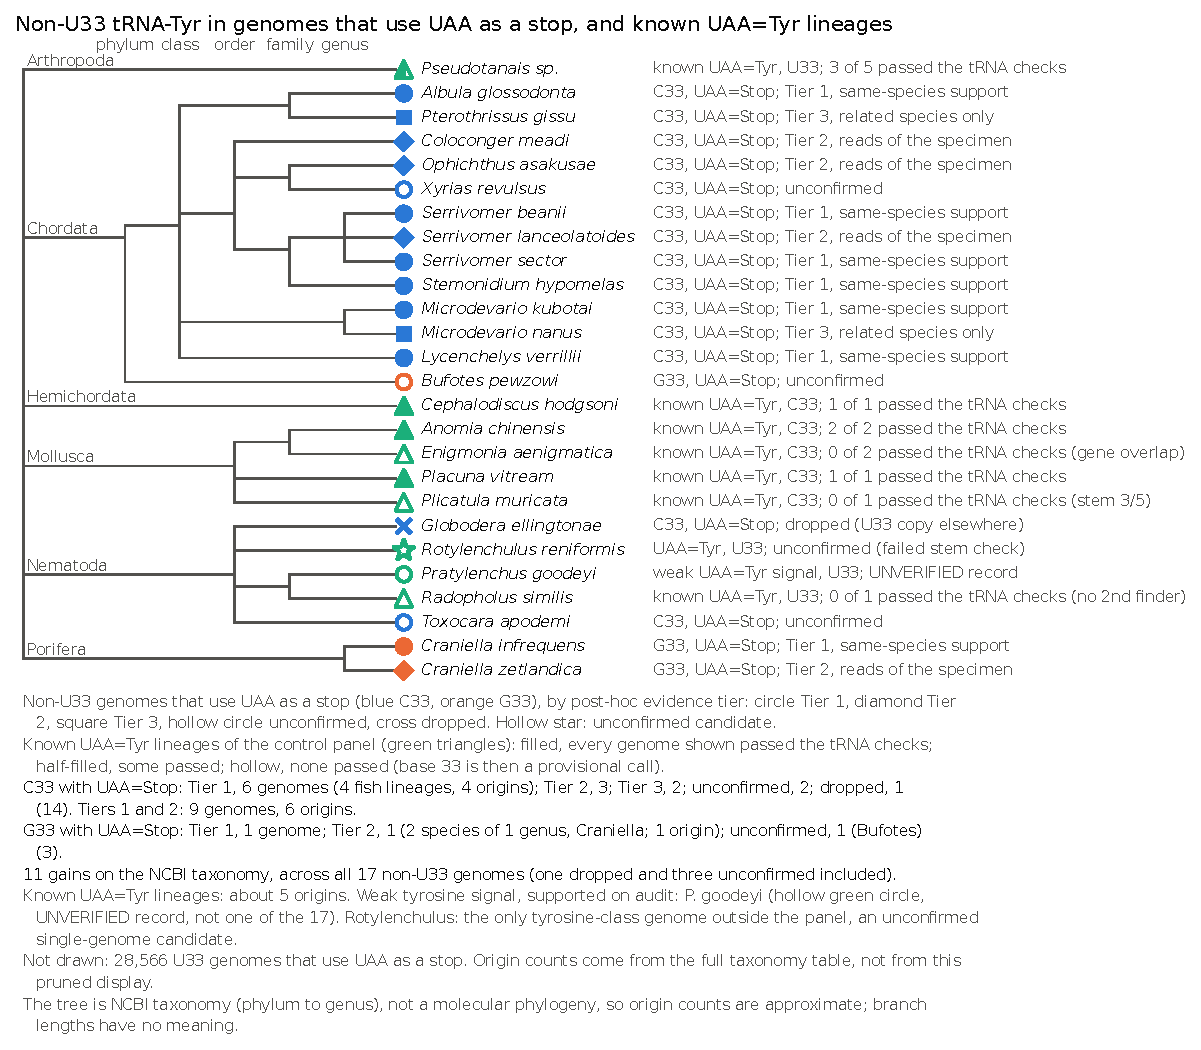
\includegraphics[width=18.2cm]{figures_v4/fig1_tree.pdf}}
\caption{\textbf{Non-U33 tRNA-Tyr(GUA) in genomes that use UAA as a stop, and the known UAA-to-tyrosine lineages, on the animal taxonomy.} Pruned NCBI taxonomy showing the 17 confirmatory genomes that use UAA as a stop and carry C33 or G33 (14 C33, 3 G33), the known reassigned lineages of the control panel, the unconfirmed single-genome candidate \textit{Rotylenchulus reniformis}, and \textit{Pratylenchus goodeyi}, a supported weak-tier record from the exploratory sweep of \texttt{UNVERIFIED} records that is not one of the 17 (hollow green circle). The 28,566 U33 genomes that use UAA as a stop are not drawn. Symbols show the post-hoc evidence tiers \texttt{[P]} (Tier 1, independent support from the same species; Tier 2, reads from the sequenced specimen; Tier 3, related species only; unconfirmed; and the dropped \textit{Globodera ellingtonae}) and, for each known reassigned species drawn, how many of its panel genomes passed the tRNA checks (species with failures include \textit{Enigmonia}, \textit{Radopholus} and \textit{Plicatula muricata}). The note ``11 gains'' gives the minimum number of gains on the NCBI taxonomy across all 17 hits, including the dropped one, counted without reversals; it does not demonstrate 11 independent evolutionary events.}\label{fig:tree}
\end{figure}

\begin{figure}[!htbp]
\centering
\makebox[\textwidth][c]{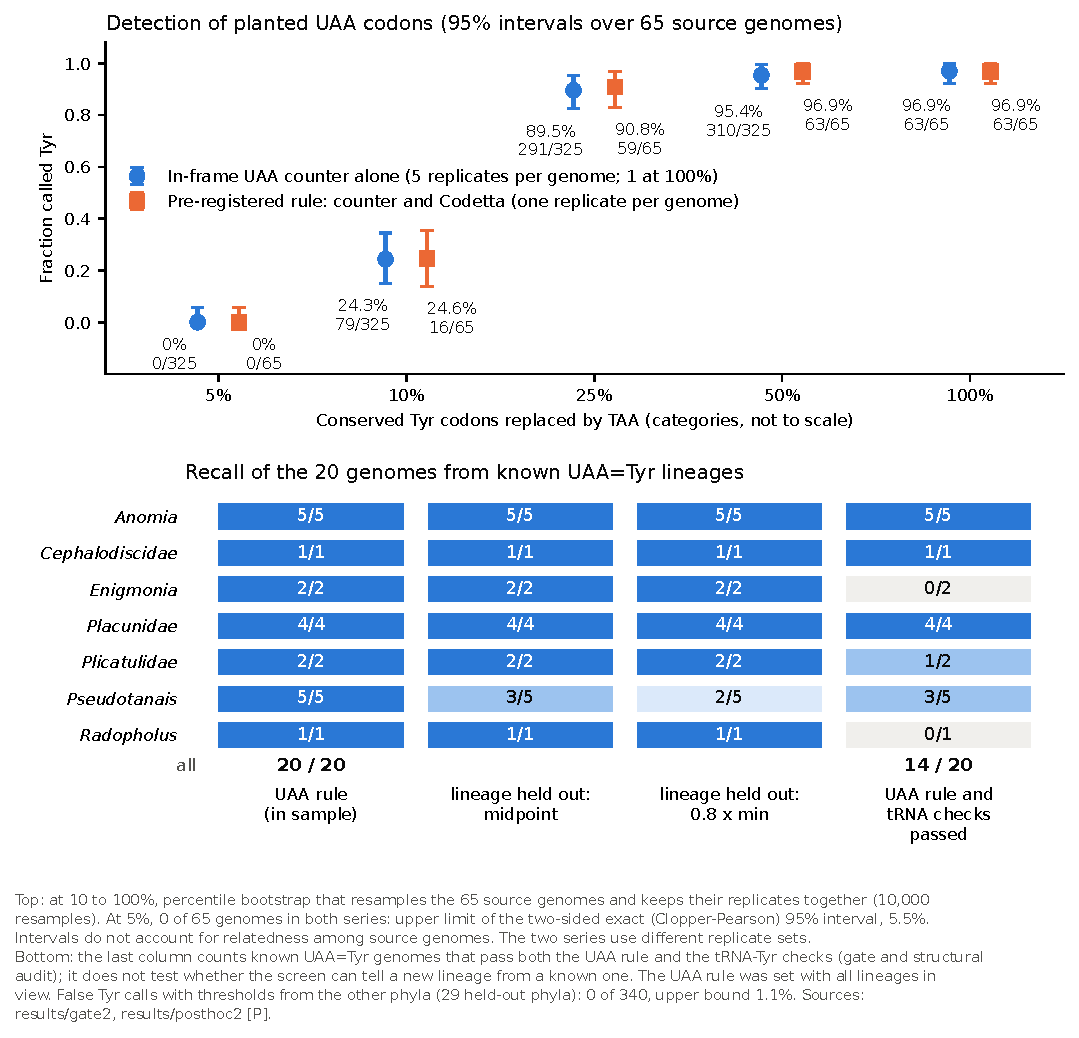
\includegraphics[width=18.2cm]{figures_v4/fig3_sensitivity.pdf}}
\caption{\textbf{Sensitivity of the UAA classifier, and recognition of known reassigned genomes by the combined criteria.} \textbf{Top:} recall in planting simulations in which 5\%, 10\%, 25\%, 50\% or 100\% of conserved tyrosine codons in 65 source genomes were replaced by TAA (categorical x-axis). The in-frame UAA counter alone (circles; 5 replicates per genome, 1 at 100\%) called 0, 24.3, 89.5, 95.4 and 96.9\% of replicates, with genome-clustered bootstrap 95\% intervals of 15.1--34.5\%, 82.5--95.4\%, 90.2--99.4\% and 92.3--100\% at 10--100\%. The pre-registered rule, counter plus Codetta (squares; one replicate per genome), called 0, 24.6, 90.8, 96.9 and 96.9\% of genomes, with intervals of 13.9--35.4\%, 83.1--96.9\%, 92.3--100\% and 92.3--100\%. At 5\%, the interval is the exact two-sided binomial 95\% upper bound on 0 of 65 genomes (5.5\%; \texttt{[P]}). \textbf{Bottom:} recall of the 20 known positives when thresholds are refitted with one lineage left out, and the number that passed both the UAA rule and the tRNA checks (tRNA-Tyr gate and structural audit): 14 of 20, against 20 of 20 for the UAA rule alone, with none passing in \textit{Enigmonia} or \textit{Radopholus}. False tyrosine calls in held-out phyla: 0 of 340 (Wilson 95\% upper bound 1.1\%; Methods).}\label{fig:calib}
\end{figure}

\begin{figure}[!htbp]
\centering
\makebox[\textwidth][c]{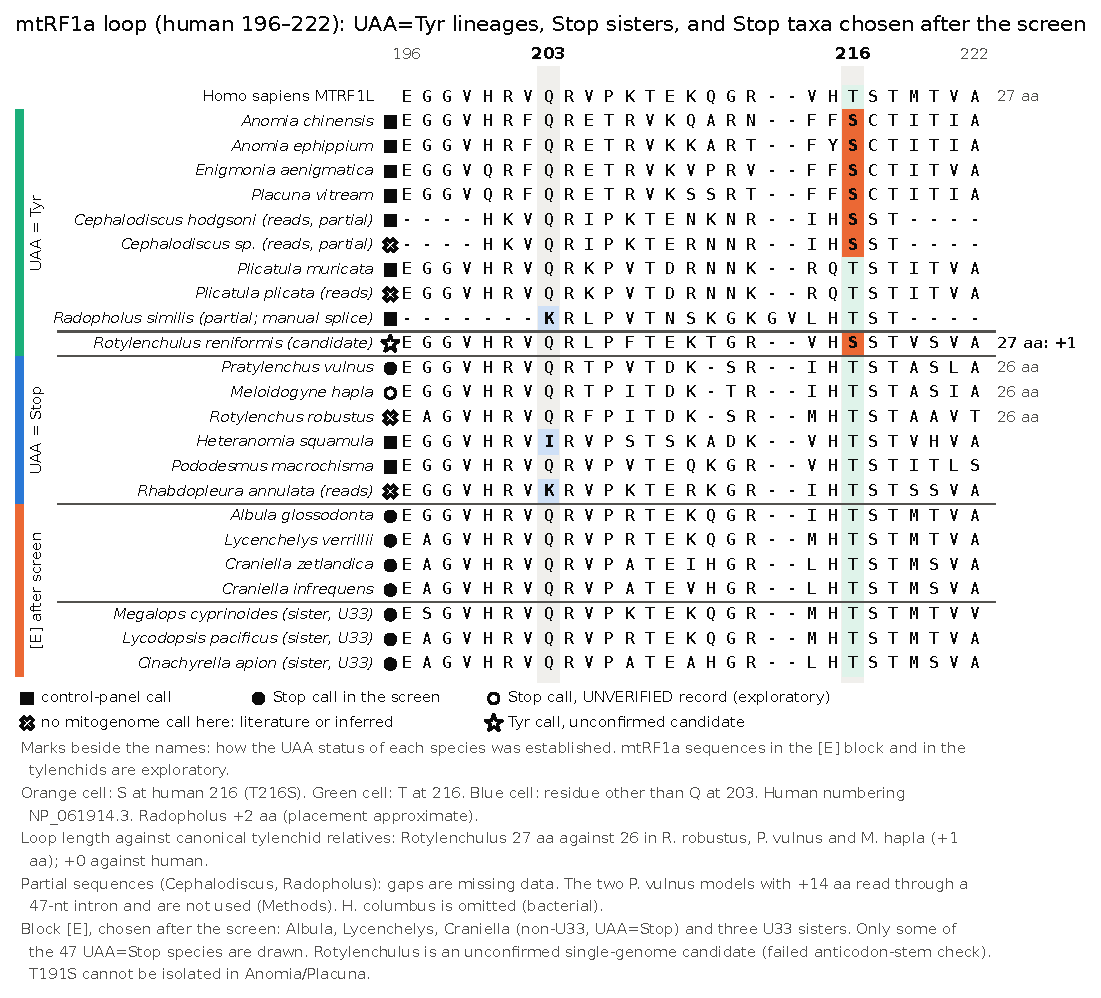
\includegraphics[width=18.2cm]{figures_v4/fig2_mtrf1a_loop.pdf}}
\caption{\textbf{The codon-recognition loop of mtRF1a and residues 203 and 216 in reassigned lineages, flagged candidates and species that use UAA as a stop.} Alignment of the loop (human \texttt{NP\_061914.3} residues 196--222, anchored on \texttt{VPxTE} and \texttt{GRxHTS}) in the known reassigned lineages (Anomiidae/Placunidae, \textit{Cephalodiscus}, Plicatulidae, \textit{Radopholus}), the unconfirmed candidate \textit{Rotylenchulus reniformis} (exploratory: Q203, S216, and a loop one residue longer than the 26-residue loops of the canonical tylenchid sisters \textit{P.\ vulnus}, \textit{M.\ hapla} and \textit{R.\ robustus}, after excluding two frameshifted $+14$ models of \textit{P.\ vulnus} that read through an intron), and species that use UAA as a stop. Only some stop-class species are drawn; 47 have both a UAA call in this study and a readable position 216, and all 47 have T216. The block labelled ``[E] after screen'' holds the species chosen after the screen for the C33 and G33 hits: those with nuclear data, and their U33 sisters. Status marks distinguish evidence classes, including taxa without a mitogenome UAA call in this study (\textit{Cephalodiscus} sp., \textit{Plicatula plicata}, \textit{Rotylenchus robustus}, and \textit{Rhabdopleura annulata}, whose stop status comes from the literature on its congener) and \textit{M.\ hapla}, a stop call from the exploratory \texttt{UNVERIFIED} sweep.}\label{fig:mtrf}
\end{figure}

% --- SUPPLEMENTARY INFORMATION OUTLINE ---
\clearpage
\section*{Supplementary Information Outline}
The following companion files from the v3 archive (\texttt{commit 35bf5df}) comprise the Supplementary Information package for bioRxiv submission:
\begin{itemize}[leftmargin=1.4em, itemsep=0.25em]
\item \textbf{Supplementary Table S1:} Terminal stops and poly(A) junctions of the six C33 fish of Section~\ref{sec:fish}, per gene (\path{results/posthoc2/sixfish_terminal_uaa.tsv}, \path{sixfish_terminal_genes.tsv}, \path{sixfish_polya_junctions.tsv}, \path{sixfish_polya_positions.tsv}).
\item \textbf{Supplementary Table S2:} Conspecific specimen metadata and \textit{COX1}/mitogenome divergence audit for the five Tier 1 fish and panel \textit{A.\ vulpes} (\path{results/posthoc2/conspecific_specimen_audit.tsv}).
\item \textbf{Supplementary Table S3:} High-copy contig search summary and non-mitochondrial contig annotations (\path{results/posthoc2/secondcopy/highcopy_summary.txt}, \path{beanii_contig.txt}, \path{contig_id_St_hypomelas.txt}).
\item \textbf{Supplementary Table S4:} Species-by-species mtRF1a denominator list (47 UAA=Stop species plus excluded \texttt{MTRF1}-only and uncalled taxa; \path{results/posthoc2/mtrf1a_stop_denominator.tsv}).
\item \textbf{Supplementary Table S5:} Phylum-stratified tRNA-Tyr completeness (\texttt{resolved}, \path{stem_audit_review}, \texttt{unresolved}, \texttt{wrong-locus}) across all 32,623 confirmatory genomes (\path{reports/REPORT.md} \S 4.3).
\item \textbf{Supplementary Table S6:} C33 in Elopomorpha and other vertebrates (\path{results/posthoc2/elopomorpha_c33.tsv}).
\item \textbf{Supplementary Table S7:} Complete per-run read-power table (all 23 primary checks and 13 competitive body-alignment checks with exact one-sided 95\% Clopper--Pearson upper bounds; \path{results/posthoc2/read_power.tsv}, \path{read_power_check4.tsv}).
\item \textbf{Supplementary Note S1:} Per-accession evidence dossiers for all 17 screen positives, \textit{R.\ reniformis}, and \textit{P.\ goodeyi} (\path{reports/dossiers/}).
\item \textbf{Supplementary Note S2:} Pre-specified \textit{R.\ reniformis} locus evaluation criteria and results (\path{results/posthoc2/roty_criteria.md}, \path{roty_eval.txt}) and \textit{Craniella} circular-mtDNA depth tables (\path{craniella_depth*.txt}).
\item \textbf{Supplementary Note S3:} Verbatim cold-review archives and item-by-item disposition tables (\path{reports/COLD_REVIEW.md}, \path{reports/COLD_REVIEW_2.md}, \path{reports/REPORT.md} \S 11 and \S 11b).
\end{itemize}

\end{document}